\documentclass[12pt,a4paper,twoside,openright]{report}
\usepackage[utf8]{inputenc}
\usepackage[T1]{fontenc}
\usepackage[margin=25mm]{geometry}
\usepackage[pdfborder={0 0 0},backref=page]{hyperref}
\usepackage{dissertation}

\newcommand{\mcandidate}{2398E}
\newcommand{\mfullname}{Skye Purchase}
\newcommand{\mcollege}{Peterhouse}
\newcommand{\mtitle}{Extracting Concepts from Simplified Graph Neural Networks}
\newcommand{\mexamination}{Computer Science Tripos -- Part II}
\newcommand{\mdate}{\today}
\newcommand{\moriginator}{\mcandidate{} \& Pietro L{\'i}o}
\newcommand{\msupervisor}{Charlotte Magister and Pietro Babiero}
\newcommand{\mwordcount}{\input{count.txt}}
\newcommand{\mlinecount}{3156}
\newcommand{\mconsent}{I am content for my dissertation to be made available to the students and staff of the University.}
\newcommand{\msignature}{Skye Purchase}

%%%%% NEW MATH DEFINITIONS %%%%%

\usepackage{amsmath,amsfonts,bm}

% Mark sections of captions for referring to divisions of figures
\newcommand{\figleft}{{\em (Left)}}
\newcommand{\figcenter}{{\em (Center)}}
\newcommand{\figright}{{\em (Right)}}
\newcommand{\figtop}{{\em (Top)}}
\newcommand{\figbottom}{{\em (Bottom)}}
\newcommand{\captiona}{{\em (a)}}
\newcommand{\captionb}{{\em (b)}}
\newcommand{\captionc}{{\em (c)}}
\newcommand{\captiond}{{\em (d)}}

% Highlight a newly defined term
\newcommand{\newterm}[1]{{\bf #1}}


% Figure reference, lower-case.
\def\figref#1{figure~\ref{#1}}
% Figure reference, capital. For start of sentence
\def\Figref#1{Figure~\ref{#1}}
\def\twofigref#1#2{figures \ref{#1} and \ref{#2}}
\def\quadfigref#1#2#3#4{figures \ref{#1}, \ref{#2}, \ref{#3} and \ref{#4}}
% Section reference, lower-case.
\def\secref#1{section~\ref{#1}}
% Section reference, capital.
\def\Secref#1{Section~\ref{#1}}
% Reference to two sections.
\def\twosecrefs#1#2{sections \ref{#1} and \ref{#2}}
% Reference to three sections.
\def\secrefs#1#2#3{sections \ref{#1}, \ref{#2} and \ref{#3}}
% Reference to an equation, lower-case.
\def\eqref#1{equation~\ref{#1}}
% Reference to an equation, upper case
\def\Eqref#1{Equation~\ref{#1}}
% A raw reference to an equation---avoid using if possible
\def\plaineqref#1{\ref{#1}}
% Reference to a chapter, lower-case.
\def\chapref#1{chapter~\ref{#1}}
% Reference to an equation, upper case.
\def\Chapref#1{Chapter~\ref{#1}}
% Reference to a range of chapters
\def\rangechapref#1#2{chapters\ref{#1}--\ref{#2}}
% Reference to an algorithm, lower-case.
\def\algref#1{algorithm~\ref{#1}}
% Reference to an algorithm, upper case.
\def\Algref#1{Algorithm~\ref{#1}}
\def\twoalgref#1#2{algorithms \ref{#1} and \ref{#2}}
\def\Twoalgref#1#2{Algorithms \ref{#1} and \ref{#2}}
% Reference to a part, lower case
\def\partref#1{part~\ref{#1}}
% Reference to a part, upper case
\def\Partref#1{Part~\ref{#1}}
\def\twopartref#1#2{parts \ref{#1} and \ref{#2}}

\def\ceil#1{\lceil #1 \rceil}
\def\floor#1{\lfloor #1 \rfloor}
\def\1{\bm{1}}
\newcommand{\train}{\mathcal{D}}
\newcommand{\valid}{\mathcal{D_{\mathrm{valid}}}}
\newcommand{\test}{\mathcal{D_{\mathrm{test}}}}

\def\eps{{\epsilon}}


% Random variables
\def\reta{{\textnormal{$\eta$}}}
\def\ra{{\textnormal{a}}}
\def\rb{{\textnormal{b}}}
\def\rc{{\textnormal{c}}}
\def\rd{{\textnormal{d}}}
\def\re{{\textnormal{e}}}
\def\rf{{\textnormal{f}}}
\def\rg{{\textnormal{g}}}
\def\rh{{\textnormal{h}}}
\def\ri{{\textnormal{i}}}
\def\rj{{\textnormal{j}}}
\def\rk{{\textnormal{k}}}
\def\rl{{\textnormal{l}}}
% rm is already a command, just don't name any random variables m
\def\rn{{\textnormal{n}}}
\def\ro{{\textnormal{o}}}
\def\rp{{\textnormal{p}}}
\def\rq{{\textnormal{q}}}
\def\rr{{\textnormal{r}}}
\def\rs{{\textnormal{s}}}
\def\rt{{\textnormal{t}}}
\def\ru{{\textnormal{u}}}
\def\rv{{\textnormal{v}}}
\def\rw{{\textnormal{w}}}
\def\rx{{\textnormal{x}}}
\def\ry{{\textnormal{y}}}
\def\rz{{\textnormal{z}}}

% Random vectors
\def\rvepsilon{{\mathbf{\epsilon}}}
\def\rvtheta{{\mathbf{\theta}}}
\def\rva{{\mathbf{a}}}
\def\rvb{{\mathbf{b}}}
\def\rvc{{\mathbf{c}}}
\def\rvd{{\mathbf{d}}}
\def\rve{{\mathbf{e}}}
\def\rvf{{\mathbf{f}}}
\def\rvg{{\mathbf{g}}}
\def\rvh{{\mathbf{h}}}
\def\rvu{{\mathbf{i}}}
\def\rvj{{\mathbf{j}}}
\def\rvk{{\mathbf{k}}}
\def\rvl{{\mathbf{l}}}
\def\rvm{{\mathbf{m}}}
\def\rvn{{\mathbf{n}}}
\def\rvo{{\mathbf{o}}}
\def\rvp{{\mathbf{p}}}
\def\rvq{{\mathbf{q}}}
\def\rvr{{\mathbf{r}}}
\def\rvs{{\mathbf{s}}}
\def\rvt{{\mathbf{t}}}
\def\rvu{{\mathbf{u}}}
\def\rvv{{\mathbf{v}}}
\def\rvw{{\mathbf{w}}}
\def\rvx{{\mathbf{x}}}
\def\rvy{{\mathbf{y}}}
\def\rvz{{\mathbf{z}}}

% Elements of random vectors
\def\erva{{\textnormal{a}}}
\def\ervb{{\textnormal{b}}}
\def\ervc{{\textnormal{c}}}
\def\ervd{{\textnormal{d}}}
\def\erve{{\textnormal{e}}}
\def\ervf{{\textnormal{f}}}
\def\ervg{{\textnormal{g}}}
\def\ervh{{\textnormal{h}}}
\def\ervi{{\textnormal{i}}}
\def\ervj{{\textnormal{j}}}
\def\ervk{{\textnormal{k}}}
\def\ervl{{\textnormal{l}}}
\def\ervm{{\textnormal{m}}}
\def\ervn{{\textnormal{n}}}
\def\ervo{{\textnormal{o}}}
\def\ervp{{\textnormal{p}}}
\def\ervq{{\textnormal{q}}}
\def\ervr{{\textnormal{r}}}
\def\ervs{{\textnormal{s}}}
\def\ervt{{\textnormal{t}}}
\def\ervu{{\textnormal{u}}}
\def\ervv{{\textnormal{v}}}
\def\ervw{{\textnormal{w}}}
\def\ervx{{\textnormal{x}}}
\def\ervy{{\textnormal{y}}}
\def\ervz{{\textnormal{z}}}

% Random matrices
\def\rmA{{\mathbf{A}}}
\def\rmB{{\mathbf{B}}}
\def\rmC{{\mathbf{C}}}
\def\rmD{{\mathbf{D}}}
\def\rmE{{\mathbf{E}}}
\def\rmF{{\mathbf{F}}}
\def\rmG{{\mathbf{G}}}
\def\rmH{{\mathbf{H}}}
\def\rmI{{\mathbf{I}}}
\def\rmJ{{\mathbf{J}}}
\def\rmK{{\mathbf{K}}}
\def\rmL{{\mathbf{L}}}
\def\rmM{{\mathbf{M}}}
\def\rmN{{\mathbf{N}}}
\def\rmO{{\mathbf{O}}}
\def\rmP{{\mathbf{P}}}
\def\rmQ{{\mathbf{Q}}}
\def\rmR{{\mathbf{R}}}
\def\rmS{{\mathbf{S}}}
\def\rmT{{\mathbf{T}}}
\def\rmU{{\mathbf{U}}}
\def\rmV{{\mathbf{V}}}
\def\rmW{{\mathbf{W}}}
\def\rmX{{\mathbf{X}}}
\def\rmY{{\mathbf{Y}}}
\def\rmZ{{\mathbf{Z}}}

% Elements of random matrices
\def\ermA{{\textnormal{A}}}
\def\ermB{{\textnormal{B}}}
\def\ermC{{\textnormal{C}}}
\def\ermD{{\textnormal{D}}}
\def\ermE{{\textnormal{E}}}
\def\ermF{{\textnormal{F}}}
\def\ermG{{\textnormal{G}}}
\def\ermH{{\textnormal{H}}}
\def\ermI{{\textnormal{I}}}
\def\ermJ{{\textnormal{J}}}
\def\ermK{{\textnormal{K}}}
\def\ermL{{\textnormal{L}}}
\def\ermM{{\textnormal{M}}}
\def\ermN{{\textnormal{N}}}
\def\ermO{{\textnormal{O}}}
\def\ermP{{\textnormal{P}}}
\def\ermQ{{\textnormal{Q}}}
\def\ermR{{\textnormal{R}}}
\def\ermS{{\textnormal{S}}}
\def\ermT{{\textnormal{T}}}
\def\ermU{{\textnormal{U}}}
\def\ermV{{\textnormal{V}}}
\def\ermW{{\textnormal{W}}}
\def\ermX{{\textnormal{X}}}
\def\ermY{{\textnormal{Y}}}
\def\ermZ{{\textnormal{Z}}}

% Vectors
\def\vzero{{\bm{0}}}
\def\vone{{\bm{1}}}
\def\vmu{{\bm{\mu}}}
\def\vtheta{{\bm{\theta}}}
\def\va{{\bm{a}}}
\def\vb{{\bm{b}}}
\def\vc{{\bm{c}}}
\def\vd{{\bm{d}}}
\def\ve{{\bm{e}}}
\def\vf{{\bm{f}}}
\def\vg{{\bm{g}}}
\def\vh{{\bm{h}}}
\def\vi{{\bm{i}}}
\def\vj{{\bm{j}}}
\def\vk{{\bm{k}}}
\def\vl{{\bm{l}}}
\def\vm{{\bm{m}}}
\def\vn{{\bm{n}}}
\def\vo{{\bm{o}}}
\def\vp{{\bm{p}}}
\def\vq{{\bm{q}}}
\def\vr{{\bm{r}}}
\def\vs{{\bm{s}}}
\def\vt{{\bm{t}}}
\def\vu{{\bm{u}}}
\def\vv{{\bm{v}}}
\def\vw{{\bm{w}}}
\def\vx{{\textbf{x}}}
\def\vy{{\bm{y}}}
\def\vz{{\bm{z}}}

% Elements of vectors
\def\evalpha{{\alpha}}
\def\evbeta{{\beta}}
\def\evepsilon{{\epsilon}}
\def\evlambda{{\lambda}}
\def\evomega{{\omega}}
\def\evmu{{\mu}}
\def\evpsi{{\psi}}
\def\evsigma{{\sigma}}
\def\evtheta{{\theta}}
\def\eva{{a}}
\def\evb{{b}}
\def\evc{{c}}
\def\evd{{d}}
\def\eve{{e}}
\def\evf{{f}}
\def\evg{{g}}
\def\evh{{h}}
\def\evi{{i}}
\def\evj{{j}}
\def\evk{{k}}
\def\evl{{l}}
\def\evm{{m}}
\def\evn{{n}}
\def\evo{{o}}
\def\evp{{p}}
\def\evq{{q}}
\def\evr{{r}}
\def\evs{{s}}
\def\evt{{t}}
\def\evu{{u}}
\def\evv{{v}}
\def\evw{{w}}
\def\evx{{x}}
\def\evy{{y}}
\def\evz{{z}}

% Matrix
\def\mA{{\bm{A}}}
\def\mB{{\bm{B}}}
\def\mC{{\bm{C}}}
\def\mD{{\bm{D}}}
\def\mE{{\bm{E}}}
\def\mF{{\bm{F}}}
\def\mG{{\bm{G}}}
\def\mH{{\bm{H}}}
\def\mI{{\bm{I}}}
\def\mJ{{\bm{J}}}
\def\mK{{\bm{K}}}
\def\mL{{\bm{L}}}
\def\mM{{\bm{M}}}
\def\mN{{\bm{N}}}
\def\mO{{\bm{O}}}
\def\mP{{\bm{P}}}
\def\mQ{{\bm{Q}}}
\def\mR{{\bm{R}}}
\def\mS{{\bm{S}}}
\def\mT{{\bm{T}}}
\def\mU{{\bm{U}}}
\def\mV{{\bm{V}}}
\def\mW{{\bm{W}}}
\def\mX{{\bm{X}}}
\def\mY{{\bm{Y}}}
\def\mZ{{\bm{Z}}}
\def\mBeta{{\bm{\beta}}}
\def\mPhi{{\bm{\Phi}}}
\def\mLambda{{\bm{\Lambda}}}
\def\mSigma{{\bm{\Sigma}}}

% Tensor
\DeclareMathAlphabet{\mathsfit}{\encodingdefault}{\sfdefault}{m}{sl}
\SetMathAlphabet{\mathsfit}{bold}{\encodingdefault}{\sfdefault}{bx}{n}
\newcommand{\tens}[1]{\bm{\mathsfit{#1}}}
\def\tA{{\tens{A}}}
\def\tB{{\tens{B}}}
\def\tC{{\tens{C}}}
\def\tD{{\tens{D}}}
\def\tE{{\tens{E}}}
\def\tF{{\tens{F}}}
\def\tG{{\tens{G}}}
\def\tH{{\tens{H}}}
\def\tI{{\tens{I}}}
\def\tJ{{\tens{J}}}
\def\tK{{\tens{K}}}
\def\tL{{\tens{L}}}
\def\tM{{\tens{M}}}
\def\tN{{\tens{N}}}
\def\tO{{\tens{O}}}
\def\tP{{\tens{P}}}
\def\tQ{{\tens{Q}}}
\def\tR{{\tens{R}}}
\def\tS{{\tens{S}}}
\def\tT{{\tens{T}}}
\def\tU{{\tens{U}}}
\def\tV{{\tens{V}}}
\def\tW{{\tens{W}}}
\def\tX{{\tens{X}}}
\def\tY{{\tens{Y}}}
\def\tZ{{\tens{Z}}}


% Graph
\def\gG{{\mathcal{G}}}
%\def\gB{{\mathcal{B}}}
%\def\gC{{\mathcal{C}}}
%\def\gD{{\mathcal{D}}}
%\def\gE{{\mathcal{E}}}
%\def\gF{{\mathcal{F}}}
%\def\gG{{\mathcal{G}}}
%\def\gH{{\mathcal{H}}}
%\def\gI{{\mathcal{I}}}
%\def\gJ{{\mathcal{J}}}
%\def\gK{{\mathcal{K}}}
%\def\gL{{\mathcal{L}}}
%\def\gM{{\mathcal{M}}}
%\def\gN{{\mathcal{N}}}
%\def\gO{{\mathcal{O}}}
%\def\gP{{\mathcal{P}}}
%\def\gQ{{\mathcal{Q}}}
%\def\gR{{\mathcal{R}}}
%\def\gS{{\mathcal{S}}}
%\def\gT{{\mathcal{T}}}
%\def\gU{{\mathcal{U}}}
%\def\gV{{\mathcal{V}}}
%\def\gW{{\mathcal{W}}}
%\def\gX{{\mathcal{X}}}
%\def\gY{{\mathcal{Y}}}
%\def\gZ{{\mathcal{Z}}}

% Sets
\def\sA{{\mathcal{A}}}
\def\sB{{\mathcal{B}}}
\def\sC{{\mathcal{C}}}
\def\sD{{\mathcal{D}}}
\def\sE{{\mathcal{E}}}
\def\sF{{\mathcal{F}}}
\def\sG{{\mathcal{G}}}
\def\sH{{\mathcal{H}}}
\def\sI{{\mathcal{I}}}
\def\sJ{{\mathcal{J}}}
\def\sK{{\mathcal{K}}}
\def\sL{{\mathcal{L}}}
\def\sM{{\mathcal{M}}}
\def\sN{{\mathcal{N}}}
\def\sO{{\mathcal{O}}}
\def\sP{{\mathcal{P}}}
\def\sQ{{\mathcal{Q}}}
\def\sR{{\mathcal{R}}}
\def\sS{{\mathcal{S}}}
\def\sT{{\mathcal{T}}}
\def\sU{{\mathcal{U}}}
\def\sV{{\mathcal{V}}}
\def\sW{{\mathcal{W}}}
\def\sX{{\mathcal{X}}}
\def\sY{{\mathcal{Y}}}
\def\sZ{{\mathcal{Z}}}

% Entries of a matrix
\def\emLambda{{\Lambda}}
\def\emA{{A}}
\def\emB{{B}}
\def\emC{{C}}
\def\emD{{D}}
\def\emE{{E}}
\def\emF{{F}}
\def\emG{{G}}
\def\emH{{H}}
\def\emI{{I}}
\def\emJ{{J}}
\def\emK{{K}}
\def\emL{{L}}
\def\emM{{M}}
\def\emN{{N}}
\def\emO{{O}}
\def\emP{{P}}
\def\emQ{{Q}}
\def\emR{{R}}
\def\emS{{S}}
\def\emT{{T}}
\def\emU{{U}}
\def\emV{{V}}
\def\emW{{W}}
\def\emX{{X}}
\def\emY{{Y}}
\def\emZ{{Z}}
\def\emSigma{{\Sigma}}

% entries of a tensor
% Same font as tensor, without \bm wrapper
\newcommand{\etens}[1]{\mathsfit{#1}}
\def\etLambda{{\etens{\Lambda}}}
\def\etA{{\etens{A}}}
\def\etB{{\etens{B}}}
\def\etC{{\etens{C}}}
\def\etD{{\etens{D}}}
\def\etE{{\etens{E}}}
\def\etF{{\etens{F}}}
\def\etG{{\etens{G}}}
\def\etH{{\etens{H}}}
\def\etI{{\etens{I}}}
\def\etJ{{\etens{J}}}
\def\etK{{\etens{K}}}
\def\etL{{\etens{L}}}
\def\etM{{\etens{M}}}
\def\etN{{\etens{N}}}
\def\etO{{\etens{O}}}
\def\etP{{\etens{P}}}
\def\etQ{{\etens{Q}}}
\def\etR{{\etens{R}}}
\def\etS{{\etens{S}}}
\def\etT{{\etens{T}}}
\def\etU{{\etens{U}}}
\def\etV{{\etens{V}}}
\def\etW{{\etens{W}}}
\def\etX{{\etens{X}}}
\def\etY{{\etens{Y}}}
\def\etZ{{\etens{Z}}}

% The true underlying data generating distribution
\newcommand{\pdata}{p_{\rm{data}}}
% The empirical distribution defined by the training set
\newcommand{\ptrain}{\hat{p}_{\rm{data}}}
\newcommand{\Ptrain}{\hat{P}_{\rm{data}}}
% The model distribution
\newcommand{\pmodel}{p_{\rm{model}}}
\newcommand{\Pmodel}{P_{\rm{model}}}
\newcommand{\ptildemodel}{\tilde{p}_{\rm{model}}}
% Stochastic autoencoder distributions
\newcommand{\pencode}{p_{\rm{encoder}}}
\newcommand{\pdecode}{p_{\rm{decoder}}}
\newcommand{\precons}{p_{\rm{reconstruct}}}

\newcommand{\laplace}{\mathrm{Laplace}} % Laplace distribution

\newcommand{\E}{\mathbb{E}}
\newcommand{\Ls}{\mathcal{L}}
\newcommand{\R}{\mathbb{R}}
\newcommand{\N}{\mathbb{N}}
\newcommand{\emp}{\tilde{p}}
\newcommand{\lr}{\alpha}
\newcommand{\reg}{\lambda}
\newcommand{\rect}{\mathrm{rectifier}}
\newcommand{\softmax}{\mathrm{softmax}}
\newcommand{\sigmoid}{\sigma}
\newcommand{\softplus}{\zeta}
\newcommand{\KL}{D_{\mathrm{KL}}}
\newcommand{\Var}{\mathrm{Var}}
\newcommand{\standarderror}{\mathrm{SE}}
\newcommand{\Cov}{\mathrm{Cov}}
% Wolfram Mathworld says $L^2$ is for function spaces and $\ell^2$ is for vectors
% But then they seem to use $L^2$ for vectors throughout the site, and so does
% wikipedia.
\newcommand{\normlzero}{L^0}
\newcommand{\normlone}{L^1}
\newcommand{\normltwo}{L^2}
\newcommand{\normlp}{L^p}
\newcommand{\normmax}{L^\infty}

\newcommand{\parents}{Pa} % See usage in notation.tex. Chosen to match Daphne's book.

\DeclareMathOperator*{\argmax}{arg\,max}
\DeclareMathOperator*{\argmin}{arg\,min}

\DeclareMathOperator{\sign}{sign}
\DeclareMathOperator{\Tr}{Tr}
\let\ab\allowbreak


\begin{document}

\bibliographystyle{plain}

%%%%%%%%%%%%%%%%%%%%%%%%%%%%%%%%%%
% Title

\thispagestyle{empty}

\rightline{\LARGE \textbf{\mfullname}}

\vspace*{60mm}
\begin{center}
    \Huge
    \textbf{\mtitle} \\[5mm]
    \mexamination \\[5mm]
    \mcollege \\[5mm]
    \mdate
\end{center}

%%%%%%%%%%%%%%%%%%%%%%%%%%%%%%%%%
% Proforma

\pagestyle{plain}

\newpage
\newpage
\section*{Declaration of originality}

I, \mfullname{} of \mcollege, being a candidate for Part II of the Computer Science Tripos, hereby declare that this dissertation and the work described in it are my own work, unaided except as may be specified below, and that the dissertation does not contain material that has already been used to any substantial extent for a comparable purpose. \mconsent

\bigskip
\leftline{Signed \msignature}
\bigskip
\leftline{Date \today}

\chapter*{Proforma}

{\large
\begin{tabular}{p{0.3\linewidth}p{0.6\linewidth}}
    Candidate Number:   & \bf \mcandidate                   \\
    Project Title:      & \bf \mtitle                       \\
    Examination:        & \bf \mexamination, 2023           \\
    Word Count:         & \bf \mwordcount\footnotemark[1]   \\
    Code Line Count:    & \bf \mlinecount                   \\
    Project Originator: & \moriginator                      \\
    Supervisor:         & \msupervisor                      \\ 
\end{tabular}
}

\note{Should I include Pietro Lio for the idea of concepts and Charlotte Magister for the paper?}

\footnotetext[1]{This word count was computed
by \texttt{texcount}
}
\stepcounter{footnote}

\section*{Original Aims of the Project}

\note{This is a first draft I am not sure what specifically should go here}

This project analyses the effect that simplifying graph neural networks has on the graph concepts that are extracted from a trained model.
It focuses specifically on the widely aclaimed Simplified Graph Convolution \cite{wu2019simplifying}[SGC] which removes the non-linearity between layers from previous graph neural network approaches reducing the problem of graph representational learning to a precomputation on the graph structure and a single linear regressor.
Using the graph concept extraction method and metrics proposed in \textit{Magister et. al} \cite{magister2021gcexplainer} the project aims to compare the concepts from trained SGC models to a baseline of Graph Convolution Network models.
Further extensions then build on SGC to see which techniques can improve accuracy and concept metrics.

\section*{Work Completed}

The project was a success. 
It fulfilled all the success criteria and further demonstrated that the Simplified Graph Convolution (SGC) does not produce as rich concepts as the Graph Convolution Network under the metrics of concept purity and completeness. 
Furthermore, it demonstrated that in the case of highly synthetic data SGC is unable to match the performance of GCN by a significant margin. 
My extensions demonstrate that in the case of real-world graph datasets, where graph structure is important, SGC continues to underperform compared to GCN and does not produce comparable concepts.
Furthermore, when extending the architecture of SGC there is significant improvement when using Jump Knowledge \note{Citation needed} techniques.
Additional work on combing SGC and GCN to gain the benefits of both systems has also proven to be successful.
However, overall SGC does not appear to be a suitable candidate for graph representational learning.
%I additionally set out to create a new parameterised dataset to further analyse the shortcomings of SGC when dealing with graph structure.
%\error{This is still not complete but I am undertaking this task.}

\section*{Special Difficulties}

None

%%%%%%%%%%%%%%%%%%%%%%%%%%%%%%%%%
% Chapters

\pagestyle{headings}

\tableofcontents

\chapter{Introduction}

% Short introduction giving a full overview

\emph{
    This dissertation explores the effect that simplifying graph neural network (GNN) architectures through linearization has on performance and graph structure awareness.
    It demonstrates that the current approach to linearising GNNs results in poor graph structure awareness but presents two novel approaches to graph representational learning in response.
    The first approach splices together a linear and non-linear GNNs into a single model and the second demonstrates accurate graph structure awareness whilst remaining quasi-linear.
%Specifically it focuses on the ideas of graph concepts which are extracted from the trained model to provide a visual demonstration of which subspaces of the input influence the model's choice of label.
%These concepts are compared to the original Graph Convolution Network (GCN~\cite{kipf2016semi}) using the metrics of concept purity and completeness proposed in \textit{Magister et al.}~\cite{magister2021gcexplainer}.
%The specific linear model chosen is the Simplified Graph Convolution (SGC) proposed in \textit{Wu et al.}~\cite{wu2019simplifying} due to claims that it matches the performance of GCN~\cite{kipf2016semi}.
%Further studies are conducted extending the basic architecture of SGC, whilst keeping with the theme of simplified graph neural networks, to see the effect on the accuracy and concept scores.
}

\section{Motivation}
\label{sec:motivation}

% Importance/rise in use of GNNs

% The rise in use of ML systems

%% Wide spread of ML systems in general prevalent in every day use

\fig{linear-vs-non-linear}{An overview of how traditional, non-linear GNNs work compared to linear GNNs. The distinction between GNN layers and graph filters is made as linearisation has focused on graph filters ignoring the more complex GNN layer approaches.}

\emph{Neural networks} (NN) are able to infer complex relationships within data, \emph{graph neural networks} (GNN) extend this functionality to connected systems where predetermined relationships exist between data points.
In these systems, such as social networks~\cite{pmlr-v70-gilmer17a} and molecules\cite{DBLP:journals/corr/abs-1806-01973}, the data can be represented as nodes connected by edges in a graph.
However, the popular deep learning approach, of multiple layers separated by non-linear activation functions, has been criticised as unnecessarily complex for these GNN architectures.~\cite{wu2019simplifying}
Instead \emph{simplified GNNs} have been proposed~\cite{chanpuriya2022simplified,chien2020adaptive,wu2019simplifying} which are either linear or quasi-linear, using one or two non-linear layers.
Figure \ref{fig:linear-vs-non-linear} demonstrates the difference in architecture between traditional, non-linear GNNs and linear GNNs.
These linear models have been shown to match the performance of non-linear GNNs on a limited number of datasets.
However, these datasets represent a small portion of possible graph datasets and little work has been done to understand how these linear GNNs work.

\fig{concept}{An example graph concept from GCN~\cite{kipf2016semi} demonstrating that when classifying the top node the model identifies the house structure and attaching arm. The consistency of the structure suggests that this is important to classifying the top node.}

The lack of understanding extends generally to NNs where explaining how a model works is largely ignored in favour of higher accuracy.
This trade-off between accuracy and explainability is not necessarily required as discussed in \textit{Zarlenga et al.}~\cite{zarlenga2022concept}.
Instead, NNs can be described by their input subspaces, referred to as \emph{concepts}, which influence the classification the most.
A precise definition of concepts is hard to define~\cite{ghorbani2019towards}, for a more in depth description see \Sref{sec:concepts}.
As an example of a graph concept, figure \ref{fig:concept} presents a concept which can be interpretted as ``a house structure with an attaching arm''.
This is more meaningful than individual node features and helps identify the importance of the house structure in classifying the highlighted green node.

The insight provided by concepts can highlight the important features of linear GNN models and provide further insight into how linearity influences graph structure awareness.
This goal motivates the project which aims to provide a deeper insight into graph representational learning and provide novel techniques to graph structure inference.

%In recent years there has been rapid development and adoption of machine learning systems such as \emph{neural networks} (NN).
%However, methods to explain how these ever larger models work is lagging behind leading to either mistrust in, or worse, blind trust in these systems.
%Though standard NNs are in the mainstream spotlight there is increasing requirement for NNs to infer knowledge about connected systems such as social networks and molecules.
%The mainstream advancements result in increasingly larger \emph{neural network} (NN) models focusing on text and image based input.
%This development makes sense from the perspective of human interaction however these are limited datastructures especially in the ever increasing interaction of digital information.
%Data present in social networks, computational biology, and systems such as smart cities have multiple predefined connections between each data point.
%In these systems the connected structure is important to classification of the individual data-points leading to the concept of \emph{graph data} and the idea of the \emph{graph neural network} (GNN).
%But criticisms of the deep learning (DL) approach to GNNs has resulted in \emph{Linear GNNs} (SGNNs) that remove non-linearity and focus on the additional information provided by the graph connections.
%\note{somewhere else: How do these linear GNNs compare to non-linear GNNs in how they infer labels for graph data?}
%\note{somewhere else: Are there potential insights into how graph structure can be better utilised?}
%\note{somewhere else: This dissertation answers these questions by evaluating an SGNN within an explanability framework and provides new methods of utilising graph data in SGNNs.}

%% Brief description of evolution of GNNs, looking at motivation and use cases

%\paragraph{Graph data}
%Rather than a dataset being only a collection of feature vectors representing observed data points within the problem setting an additional adjacency matrix is also present.
%The adjacency matrix represents the connections between data points that is inherently present in the observed data.
%An example being friendship connections in a social network or bonds between atoms in a molecule.
%This additional structure provides useful information for tasks where the interaction between data points has importance to the data points themselves.
%More complex graph data may also include attributes associated with the connections which can be simple scalars or multidimensional vectors.
%For these reasons graph data is a highly flexible and versatile datastructure promoting complex inference.

%\paragraph{Graph neural networks (GNNs)} 
%are designed to handle graph data where the connections between data points is an important aspect as the data itself.
%The standard form of a GNN 
%\note{make sure this is valid here!}
%consists of multiple layers connected together by a non-linearity step.
%Each layer performs inference on a node's feature vector in the same way as a NN would perform inference.
%The graph structure is utilised by broadcasting this new node representation along the connected edges to neighbouring nodes.
%Each node then aggregates the representations of its neighbouring nodes creating a compact representation of the neighbourhood according to itself.
%The updated representation and aggregation are then combined to produce a final representation before the next layer.
%By using a process known as \emph{message passing} each node's feature vector is updated based on the graph neighbourhood inferring graph structure as well.
%This process, known as \emph{message passing}, allows a GNN to utilise the graph structure and infer more complex relationships between the data points than an ordinary NN.

%% Rapid integration of these systems 

% The lack of clarity in ML systems
% -> Explainability
% -> Concepts

%\paragraph{Linearising NNs}
%Modern specialist computer hardware, such as graphics processing units (GPU), are incredibly efficient at carrying out large linear operations such as matrix multiplication.
%However, the vast majority of NNs contain non-linear operators between generally linear layers.
%The idea of linearising NNs is to remove \emph{some} of the non-linearity in the architecture multiple layers to be combined into a single linear operation.
%Removal the early non-linearity (or all the non-linearity) results in a pre-computation step that can be carried out on an entire dataset before training or inference.
%%Thus in cases where inputs are sampled from a collection of data points this prevents calculating the same operation on the same data point across samples.
%But, it is important that this does not effect the performance of the model.

%\paragraph{Linear GNNs}
%The process of message passing though complex conceptually can easily be decomposed into a linear operation on the graph features and graph adjacency.
%Using the idea of linearising NNs the non-linearity between individual message passing layers can be removed.
%This allows a GNN to pre-compute multiple message passing steps on the graph dataset before inference.
%Inference then results in a simple classification or linear regression task where only a single layer is required.
%This new \emph{linear GNN} (SGNN) remove their non-linear complexities whilst demonstrating comparable performance to standard GNNs.

%\paragraph{Explainability}
%The advancement of new NNs has focused on improving the performance in metrics such as accuracy and training cost which has resulted in impressive models.
%However, these models remain as blackboxes to the users of these systems but equally to the designers.
%Once a model is trained on a specific dataset there is very limited understanding of how the model is analysing the input to produce a result.
%This can and does create a lot of mistrust in NNs as there is a large element of trusting that the output it produces on unseen data will match our expectation.
%The idea of explainability is to provide different methods of visualising how a model works to a human as a form of verification or to provide insight.
%Many different approaches exist including before, during and after training, to varying degrees of explanation.

%% Importance of understanding ML inference
%% -> Link to potential use cases 

%% Issues with interfering with training

%% Recent development in developing frameworks to analyse these aspects
%% The different goals of explainability 

%\paragraph{Concepts}
%A specific form of explainability that is applied after the training of a model \note{Check that this is always the case!} is that of concepts.
%The idea is to find different subspaces of the input space (where each input to tthe NN is some element of the input space) that correspondent to a specific output.
%This way patterns can be found between input and output to verify that the model is behaving as expected.
%In this dissertation the focus is on graph concepts which are subgraphs created from the input graph(s) for the model.
%These subgraphs represent the graph structures that the model is using to carry out inference on specific inputs.
%
%\paragraph{Concepts in simplified GNNs}
%Though SGNNs show competitive performance when looking at classification accuracy they are a black box as with the majority of NNs.
%As SGNNs delay the influence of the models weights until the final classification step this provides an opportunity to see how graph concepts are effected.
%If these models are truly comparable to GNNs then the concepts should demonstrate how the message passing steps operate.
%These results could therefore influence the design of future networks as the DL approach may not be required for graph data. \note{This needs better wording, I don't know how much I agree with it myself.}

%% The idea of a concept
%% The fact in our case this is done after training
%% -> This does not effect training performance

% More efficient systems should not sacrifice ease of understanding

\section{Previous and Related Work}
This project focuses on two different areas of graph representational learning: explainability and linearisation.
Within graph explainability there have been many different methods presented to explain how GNNs work.

\textit{Ying et al.}~\cite{ying2019gnnexplainer} identifies subgraphs as ideal explainability tools for GNNs. 
%Subgraphs are generated by perturbing the input graph and comparing the model predictions to the original predictions.
%By maximising mutual information it identifies important structures and node features in the input which can be masked to generate subgraphs.
However, their approach focuses on perturbing the input graph resulting in local explanations for each classification rather than desired global explanations.
\textit{Luo et al.}~\cite{luo2020parameterized} combat this by learning optimal perturbations from the edge embeddings thus providing global explanations.
Both techniques learn an additional model to explain the GNN on a specific graph instance.

Instead, \textit{Magister et al.}~\cite{magister2021gcexplainer} provide global, model-level explanations by producing graph concepts.
Concepts are human-interpretable units~\cite{ghorbani2019towards}, in the case of graph concepts these are best represented by subgraphs as demonstrated in figure \ref{fig:concept}.
The method achieves this by adapting \textit{automatic concept extraction}~\cite{ghorbani2019towards} to GNNs to extract graph concepts.
%Rather than perturb the input the model's predictions are clustered based on similarity and subgraphs are generated by considering a node's neighbourhood.
%They present two metrics, purity and completeness, to compare different clusterings and identify the optimal subgraphs.
\textit{Magister et al.} apply this method to GCN~\cite{kipf2016semi}, a non-linear GNN, this project extends the work and applies the method to a linear GNN providing a comparison between the two architectures.

Within GNN linearisation multiple architectures have been proposed focusing primarily on linearising GCN~\cite{kipf2016semi}.

\textit{Wu et al.}~\cite{wu2019simplifying} proposed the original linearised GNN, SGC, by removing the non-linearity from the GCN~\cite{kipf2016semi} architecture.
%The argument is that the non-linearity in GCN is derived from the current NN research at the time and that this approach was unnecessary.
By removing non-linearity SGC removes the redundant computation of activation functions resulting in a fixed pre-computation and learnable classifier.
SGC is chosen as the linear model to compare to the non-linear GCN, furthermore the proposed SGCN (\Sref{sec:SGCN}) extends SGC by reintroducing some non-linearity from GCN.

\textit{Chanpuriya et al.}~\cite{chanpuriya2022simplified} propose adaptive SGC (ASGC) which introduces learnable parameters to the pre-computation allowing the model to adapt to heterophilic data.
\textit{Chien et al.}~\cite{chien2020adaptive} identify heterophilic data as a general problem and propose generalised pagerank GNN (GPR-GNN) as a solution.
Both SGC and ASGC are special cases of GPR-GNN where the proposed node representation NN is removed.
%\textit{Chien and Peng} suggest learning hidden node representation using a standard NN and then propagate these features using generalized pagerank.
The proposed JSGC (\Sref{sec:Jump-SGC}) is closely related to GPR-GNN removing the node representation NN and replacing GPR with jumping-knowledge networks~\cite{xu2018representation}.

%This project is based on the recent work by \textit{Magister et al.}~\cite{magister2021gcexplainer} which proposes a new method to extract graph concepts and introduces two concept metrics to compare between extracted concepts.
%Using these metrics a linear GNN and its non-linear counterpart are compared to provide more insight into the effect of linearisation.
%
%The project also implements and extends the work by \textit{Wu et al.}~\cite{wu2019simplifying} who introduce \emph{simplified graph convolution} (SGC)
%The method linearises the graph convolution layers in the network allowing these to be pre-computed.
%This linear architecture will be used to compare against the non-linear GCN~\cite{kipf2016semi} counterpart.
%
%\textit{Chanpuriya et al.}~\cite{chanpuriya2022simplified} demonstrate that SGC achieves poor performance on heterophilic data and introduces SGC with heterophily to overcome these issues.
%\textit{Navarin et al.}~\cite{navarin2020linear} introduce two new linear GNN architectures the introducing exponential and linear parameterised pre-computations.
%This project presents two additional approaches to improving the performance of SGC.

\section{Contributions}

This project applies the graph explainability tools proposed by \textit{Magister et al.}~\cite{magister2021gcexplainer} to the linear model SGC \cite{wu2019simplifying}.
This provides a new analysis of linear GNN models and their limitations providing new insight into how graph structure is inferred.
These results demonstrate that purely linear models, such as SGC, cannot infer fine-grained graph structure.
The lack of graph structure awareness suggest the SGC is primarily focused on tabular data rather than graph data.

Two novel extensions are proposed to improve the accuracy and graph structure awareness of SGC.
\begin{enumerate}
    \item
        A new model which uses SGC pre-computation with GCN~\cite{kipf2016semi} layers to utilise the efficient pre-computation with the high accuracy GCN layers.
        The architecture removes unnecessary non-linearity from the initial layers of a GCN model by finding an SGC pre-computation that closely resembles the GCN latent space.
        This means that the effect on the final layers of the GCN model is minimised.
    \item
        A new architecture which uses SGC within an adaptation of jumping knowledge networks~\cite{xu2018representation}.
        The architecture aggregates each successive SGC pre-computation so that the model has more control of the node representations.
        This improves the graph structure awareness of SGC whilst remaining quasi-linear.
\end{enumerate}
Both approaches are successful in increasing both graph structure awareness and accuracy demonstrating that graph structure awareness is achievable whilst remaining quasi-linear.


\chapter{Preparation}

\section{Background}

\section{Graph Representational Learning}

\subsection{Graph Neural Networks}

\subsection{Graph Convolutional Network}

\subsection{Simplified Graph Convolution}

\section{Explainability}

\subsection{Concepts}

\subsection{Graph Concept Explainer}

\section{Datasets}

\subsection{Synthetic}

\subsection{Real-World}

\section{Tools Used}

%MAYBE THE REQUIREMENTS ANALYSIS POST-HUMOUSLY?

\section{Software Methodology}

\section{Testing}

\section{Licensing}

\section{Starting Point}

\chapter{Implementation}

\section{Datasets}
\label{sec:datasets-imp}
\Sref{sec:datasets-theory} presents several datasets that cover a range of different GNN training styles and motifs.
The inductive datasets discussed in \Sref{sec:RWD} are already packaged and available through \texttt{PyTorch Geometric}~\cite{Fey/Lenssen/2019} as well as the Planetoid~\cite{planetoid,citation} datasets.

\paragraph{Synthetic datasets}
The synthetic datasets discussed in \Sref{sec:synth} are available pre-built on GitHub and \texttt{PyTorch Geometric}~\cite{Fey/Lenssen/2019} provide limited versions of a small subset.
Rather than use these the datasets are reimplemented to allow for more rigorous testing described in \Sref{sec:testing-imp}.

%The motifs described in \Sref{sec:synth} can be hard-coded.
%each motif is therefore an adjacency matrix (in coordinate form) and a label vector.
When generating the dataset the base graph adjacency is generated first. 
%with a label vector assigning every node to class 0.
%The Barabasi-Albert graph is generated probabilistically adding one node at a time and connecting each node to the existing graph based on the degree of the nodes currently in the graph.
Then the hard-coded adjacency for each motif required is 
%the hard-coded tensors are adjusted and 
appended to the ongoing adjacency matrix and label vector by connecting
%This adjustment includes adding an additional bidirectional connection between 
a random node in the base graph to a predetermined node of the motif.

The datasets need to be compliant with \texttt{PyTorch Geometric} to be used correctly and so must extend the \texttt{InMemoryDataset} abstract class. 
This is designed for datasets that are small enough to be generated and stored within RAM.
%As these are transductive datasets as described in \Sref{sec:datasets-theory} 
Each dataset contains a single graph \texttt{Data} object is created that is then accessed through a data loader.

The \texttt{Data} object includes train and test split masks randomly assigning nodes to achieve an 80:20 ratio based on the seed value.
%This random assignment is based on the seed value for the experiment discussed in \Sref{sec:reproducibility}.
%randomness also applies to the generation of the graph 
This creates significantly different graphs for each generation meaning that nodes for one seed value are unseen for a different seed value.

\section{Models}
\label{sec:models}

\texttt{PyTorch Geometric}~\cite{Fey/Lenssen/2019} provides an abstract \texttt{MessagePassing} class which defines a generic GNN layer.
\texttt{MessagePassing} extends the \texttt{PyTorch}~\cite{paszke2019pytorch} \texttt{Module} class adding the \texttt{message\_passing} method which is called during the \texttt{forward} method passing node representations and associated adjacency.
This method allows the implementation of the function
\begin{equation}
    \mH^{(l+1)} = \mS\mH^{(l)}\bm{\Theta}^{(l)},
\end{equation}
described in \ref{sec:GCN} as equation \ref{eq:GCN1}.
During the \texttt{message\_passing} method the normalised adjacency $\mS$ is applied to the node representations $\mH^{(l)}$.
After \texttt{message\_passing} a linear layer is applied to the representations.

These GCN layers (provided by \texttt{PyTorch Geometric}) can then be combined with a ReLU activation function to form a GCN model.
In comparison, SGC needs only to be a classifier as explained in \Sref{sec:datasets-imp} and so contains a single linear layer.

\subsection{SGC}
The majority of SGC is the pre-computation
\begin{equation}
    \label{eq:pre-comp}
    \mS^k\mX
\end{equation}
of equation \ref{eq:SGC} where $\mS$ is the filter defined in equations \ref{eq:op} and \ref{eq:norm}.
As $\mS$ 
%is defined in terms of the adjacency matrix which 
does not change during training equation \ref{eq:pre-comp} can be applied before training.
This process is achieved with three functions that calculate the normalised filter $\mS$,
%by computing the required matrices and multiplications, 
convert the matrix form and successively apply the filter to the node representations.

This results in a new feature matrix which replaces the original \texttt{Data} object's features.
Equation \ref{eq:SGC} shows that SGC does not need any adjacency information and can instead be implemented as a classifier.
For consistency and the concept evaluation functions described in \Sref{sec:concepts} the adjacency matrix is kept.
%A new \texttt{Data} object is created copying the labels, data splits and adjacency of the input graph but with the pre-computation matrix as the feature matrix.

\section{Machine Learning Pipeline}
\label{sec:pipeline}

The ML pipeline is the infrastructure that links the datasets, pre-computation, data loaders, and models together to train and evaluate the models.
This allows for specific experiment configurations to be run changing each component individually or together.
As the main aspect of this project is concept extraction, evaluation, and interpretation I use \texttt{PyTorch Lightning}~\cite{Falcon_PyTorch_Lightning_2019} as the main component of the pipeline.

\texttt{PyTorch Lightning} provides \texttt{Lightning Modules} that act as wrappers around standard \texttt{PyTorch}~\cite{paszke2019pytorch} (and therefore \texttt{PyTorch Geometric}~\cite{Fey/Lenssen/2019}) modules and carry out all the required training, validation and testing loops.
Unfortunately, for the core project and extensions, a single wrapper is not possible.
This is because the wrappers need to behave differently for SGC and GCN as GCN needs additional adjacency information.
Additionally, the real-world graph classification datasets require one-hot encoding when calculating loss whereas the synthetic datasets do not.
Therefore the project implements 5 different wrappers.

The datasets, pre-computation and data loaders discussed in \Sref{sec:datasets-imp}, the models described in \Sref{sec:models} are controlled by \texttt{main.py}.
To run a single experiment the specific model build, dataset, seed, save destinations, etc. need to be passed to this function.
To reduce this overhead multiple bash scripts are dynamically created to run single quick experiments or full experiments which test the model on prechosen random seeds.

\subsection{Reproducibility}
\label{sec:reproducibility}
It is important that all the results presented in \Sref{ch:evaluation} can be replicated later.
%This is both for the results presented in this dissertation but also for results found during experimentation in the extension phase.
To achieve this every experiment must set a seed value which is saved along with the results.
%This way when running the same configuration again using the same seed the expected outcome should be the same within very small bounds.
Furthermore, the results achieved are linked to the model build which specifies details of the model so that it can be replicated.
%that identifies all the hyperparameters used.
%The model build 
%in a completely different ML pipeline.
Thus the build files need to be human-readable and easily expandable.

To achieve these two requirements YAML files are used as they are very readable and integrate with the rest of the pipeline.
Each build has a unique YAML file following the convention \texttt{<model>.<dataloader>.<dataset>.<version>.yml}.
Storing the YAML filename, seed and timestamp with every set of results allows for accurate reproduction.

\subsection{Experimentation}
The infrastructure used in \Sref{sec:reproducibility} also aids experimentation by linking results to configurations.
This is particularly desirable during the extension phase where the best method is unknown.

Finding the optimal hyperparameters is essential as incorrect hyperparameters can lead to artificially low performance and thus invalidate the interpretation of the models.
To find hyperparameters \texttt{sweep.py} takes a set of different hyperparameter values and runs a short evaluation of the performance.
To properly evaluate models this evaluation mustn't use nodes that are in the final test set.
As discussed in \Sref{sec:datasets-imp} choosing different seeds means that nodes in the evaluation test set are unseen.

\section{Concept Extraction and Evaluation}
\label{sec:concepts}

\subsection{Extraction}
\label{sec:extraction}

This subsection uses the idea of \emph{activation spaces} which are multidimensional spaces within which the node representations after an activation layer are expressed.\footnote{The term activation space, though incorrect, is also used when referring to SGC pre-computation to avoid confusion.}
The concept extraction discussed in \Sref{sec:GCE} requires storing and then clustering this activation space.
These occur at different points with storing occurring during the experiment run and clustering occurring afterwards.

\paragraph{Storing}
SGC and GCN behave differently in regards to storing activation spaces as SGC pre-computes the node representations whereas GCN calculates them during training.

In SGC the node representations from each successive filter application can be stored in a dictionary and written out.
This allows for multiple layers to be analysed without training which in turn can be used to optimise SGC before training.

In comparison, GCN requires a function during the forward pass of the model to save the node representations.
\texttt{PyTorch}~\cite{paszke2019pytorch} provides this functionality through \emph{hooks} which are functions that can be attached to modules.
This function will then run whenever the modules \texttt{forward} method is run and \texttt{PyTorch} will pass the input, output and module to the function.
A hook function is created which saves the output of a layer to a dictionary, the dictionary is written to a file after the test loop is complete.
%this means that the activations represent the final model.

\paragraph{Clustering}
%The described activation dictionaries can be loaded and
For each of the layers, the node representations are clustered using $k$-means as it is the best-performing model as seen in \textit{Magister et al.}~\cite{magister2021gcexplainer}.
The specific implementation of $k$-means is provided by
%Rather than implement my own $k$-means algorithm I utilise the algorithm already present within
\texttt{scikit learn}~\cite{scikit-learn}.
The clustering is parameterised by the number of clusters which
can be chosen based on the concept scores in \Sref{sec:GCE}.
%can then motivate the choice of this value
Though focusing on maximising completeness will not necessarily lead to better concepts.

The example subgraphs are generated by a breadth first search of a clustered node's neighbourhood up to a given depth.
The depth of the search is determined by the node's receptive field which determines how many hops between connected nodes are allowed.

\subsection{Evaluation}
\label{sec:concept-eval}

Once the concepts are extracted using the methods detailed in \Sref{sec:extraction} the two concept metrics can be calculated.
The concepts from a model are extracted from each layer using the same clustering and receptive field constants provided.
The theory behind the two concept metrics of completeness and purity are outlined in \Sref{sec:GCE}.

\paragraph{Completeness}
As discussed in \Sref{sec:GCE} completeness is determined by whether the extracted concepts can be used to infer node labels.
This is achieved by fitting a decision tree~\cite{kazhdan2020now} as proposed by \textit{Magister et al.}~\cite{magister2021gcexplainer} to the concepts and labels.
The accuracy of this decision tree on the hold-out test set represents the completeness of the concepts extracted.

The decision tree predicts a label for each of the nodes in the graph based on the concept that the node belongs to.
The input data is therefore the predicted clusters for each of the nodes based on the $k$-means clustering.
The target is constructed from the node labels for each node in the input.

\paragraph{Purity}
To calculate the purity the three quintessential subgraphs of each concept are chosen.
Each quintessential subgraph is chosen based on the distance to the concept centroid and is constructed by a breadth-first search from the subgraphs node of interest.

The purity is calculated by taking the average of the GED described in \Sref{sec:GCE} between these subgraphs.
The graph edits that are allowed are adding or removing a node or edge ignoring the node representations.
Thus coherence of a concept is based on graph structure rather than node representations, this drawback is discussed further in \Sref{sec:concept-analysis}.

Three quintessential graphs are considered due to the computational cost of calculating GED.
In the cases where the number of nodes in a subgraph exceeds 13 the purity calculation is skipped.
This can be mitigated by calculating an upper bound on the GED in $\mathcal{O}(n^3)$ however this would negatively impact the purity scores of Barabasi-Albert concepts.

\subsection{Visualisation}
\label{sec:vis}
The visualisation of the concepts uses the same subgraph construction as purity in \Sref{sec:concept-eval}.
However, more quintessential graphs may be considered to better visualise the extracted concepts.
This means the visual results may contradict the purity score as subgraphs further from the centroid may not match the calculated purity.

For the synthetic graphs, the subgraphs are coloured with two colours, green indicating the node of interest and pink indicating neighbouring nodes.
In some instances, one subgraph may contain a node of interest in another subgraph resulting in multiple green nodes appearing in both.
%This represents the fact that the model does not distinguish between these nodes within the graph structure.
The same process is used for REDDIT-BINARY~\cite{Morris+2020}.

In the case of Mutagenicity~\cite{Morris+2020} \textit{Magister et al.}~\cite{magister2021gcexplainer} assign a unique colour to each atom within a concept meaning that between concepts the colour scheme does not match.
To provide a better comparison between concepts a chemical colour scheme is chosen and each node is coloured according to this.

Regardless of the dataset, each subgraph is titled by the label of the node of interest.
This provides additional information about the coherence of the concept labels.

\section{Testing}
\label{sec:testing-imp}
As discussed in \Sref{sec:testing} the project utilises two forms of testing to verify the implementation.
Additionally, the pipeline (described in \Sref{sec:pipeline}) verifies that the modules integrate correctly.

\paragraph{Unit testing}
Three components of the software follow traditional software development and therefore unit tests are used:
\begin{itemize}
    \item[] 
        \smalltitle{Synthetic datasets} 
        These have strict defining properties based on the parameters passed during initialisation.
        Verification of the datasets can be done with hard-coded values for small initialisations and
        %to verify the correct motif is used or base graph.
        general properties for larger instances.
        %properties such as the expected number of nodes, number of classes, and number of nodes within a given class can be
    \item[] 
        \smalltitle{Pre-computation}
        This has already been verified through the derivation in \Sref{sec:GCN} and \Sref{sec:SGC}.
        Small test graphs are used to verify that these are correctly implemented.
    \item[] 
        \smalltitle{Concept evaluation}
        %Though parts of this implementation use algorithms provided by \texttt{scikit learn}~\cite{scikit-learn} the results of these functions needs to be verified in the new context.
        Small graphs with pre-determined clusters verify the implementation by comparing the predicted clusters to the expected clusterings.
        In the case of purity isomorphic graphs and non-isomorphic of known GED are used.
\end{itemize}

\paragraph{Reproduction of prior results}
for both \textit{Magister et al.}~\cite{magister2021gcexplainer} and \textit{Wu et al.}~\cite{wu2019simplifying} are presented in \Sref{sec:reproduction}.
The hyperparameters used are available in \Aref{app:hyperparameters}.

\section{Extensions}
\label{sec:extensions-imp}
After completing the core project my extensions focus on improving the low performance demonstrated by SGC in \Sref{sec:comp-acc}.
The motivation for the following extensions is based on the results of the core project.
This section outlines the three extensions completed, the motivation for each and the implementation details.
The evaluation of the extensions is presented in \Sref{sec:extension-eval}.

\subsection{SGC graph classification}
\paragraph{Motivation}
The datasets used in \textit{Magister et al.}~\cite{magister2021gcexplainer} include two real-world datasets focusing on graph classification.
%As discussed in \Sref{sec:datasets-theory} these graph classification datasets are also inductive rather than transductive which provides another test of the capabilities of SGC.
Furthermore, though \Sref{sec:comp-acc} suggests SGC performs poorly, this could be because of the synthetic nature of the datasets.

\paragraph{Prior work}
\textit{Wu et al.}~\cite{wu2019simplifying} discuss graph classification for SGC and suggest replacing GCN in a deep graph convolutional neural network~\cite{zhang2018end}.
In comparison \textit{Magister et al.}~\cite{magister2021gcexplainer} utilise pooling on the graph node representations from a GCN to achieve graph classification.
%The label of the entire graph can then be inferred from this single representation.
The latter method is chosen as it allows for a fairer comparison between SGC and the results achieved by \textit{Magister et al.}.

\paragraph{Implementation}
The new SGC model has an additional pooling layer to create a single representation for each graph.
Each graph now has a single label with no node labels, given that concept extraction is done on the node level the method proposed in \Sref{sec:concept-eval} does not work.

This is solved by broadcasting the graph label to each of the nodes in the graph allowing the graphs to be combined into a disconnected forest of graphs which can be clustered.
Calculation of concept scores and the visualisation of a concept remains the same as that presented in \Sref{sec:concept-eval} and \Sref{sec:vis}.

\subsection{SGC and GCN mixed model}
\label{sec:SGCN}
\paragraph{Motivation}
The benefit of SGC is to reduce the complexity of GCN and pre-compute the successive applications of the graph filter, described in equations \ref{eq:op} and \ref{eq:norm}, by removing the non-linearity between layers.
This pre-computation reduces the cost of training a model as it can be calculated before training unlike in GCN.

However, due to the low accuracy of SGC in comparison to GCN, seen in \Sref{sec:comp-acc}, some properties of GCN must be required to achieve high accuracy.
Utilising both the SGC pre-computation and GCN layers, referred to as SGCN, could therefore yield a high-accuracy model with fast pre-computation.

\paragraph{Implementation}
For simplicity and to utilise the pre-computation SGCN starts with SGC layers followed by GCN layers.
For a fair comparison, the total number of layers remains the same as the corresponding SGC and GCN models.
This reduces the problem of finding where SGC and GCN agree the most.

This is achieved using \emph{adjusted mutual information}(AMI) between the two models.
Mutual information gives a measure for the dependence of the two models' clusters and therefore how similar the models are.
However, this does not take into account the random chance of two nodes appearing in the same cluster.
Therefore the mutual information is adjusted for this chance resulting in a number in the range $[0, 1]$ where $1$ represents identical clustering.

To better visualise the resulting model the activation space of the models is reduced using \emph{t-distributed stochastic neighbour embedding} (t-SNE) to 2 dimensions.
This clusters similar representations together allowing these clusters to be compared to see why a specific layer has the highest AMI.

\subsection{Jumping knowledge SGC}
\paragraph{Motivation}
\Sref{sec:concept-analysis} discusses the limited influence that SGC has on node representations.
This is because an SGC model, of degree $k$, can only infer graph structure from the aggregated node representations within $k$ hops.
In comparison, GCN can manipulate node representations and can therefore infer structure from each $k$-depth neighbourhood.
This suggests that the low accuracy seen in \Sref{sec:comp-acc} and poor graph structure awareness seen in \Sref{sec:comp-concept} may be due to the linearity or lack of influence.

Therefore the novel \emph{jump-SGC}(JSGC) is proposed which provides the classifier with node representations from each degree of the pre-computation.
This idea mimics \emph{jumping knowledge networks} (JKNs) proposed by \textit{Xu et al.}~\cite{xu2018representation} hence the name ``jump''.

\paragraph{Prior work}
\textit{Xu et al.}~\cite{xu2018representation} identify the drawbacks of node aggregation in accurately representing the neighbourhood of a node.
They propose aggregating the node representations after successive neighbourhood aggregation layers together to provide a better representation.
Three main methods of aggregation are proposed but, given the small size of the datasets, the concatenation method is chosen.

By concatenating successive neighbourhood aggregations and then reducing the dimensionality uniform influence across all $k$-depth neighbourhoods is achieved.
This is because the detail present in the smaller neighbourhoods can be combined with the wider awareness of larger neighbourhoods.

\paragraph{Implementation}
For JSGC this leads to two changes to the pre-computation and model.
During pre-computation successive applications of the normalised filter are concatenated together.
A linear layer is then added to the standard SGC to reduce this concatenated dimension, during this JSGC can infer more complex graph structures than SGC.
To combine this with the classifier a single non-linear rectified linear unit layer is introduced.
This non-linearity remains constant regardless of how the model scales and therefore it is deemed negligible.

\section{Repository}

\begin{figure}
\dirtree{%
.1 \myfolder{black}{}.
.2   \myfolder{red}{README.md}.
.2   \myfolder{red}{requirements.txt}.
.2  \myfolder{blue}{activations.................................extracted activation space}.
.2  \myfolder{blue}{checkpoints..........................................model checkpoints}.
.2  \myfolder{blue}{data...............................................downloaded datasets}.
.2  \myfolder{blue}{output...............................model accuracy and concept output}.
.3  \myfolder{blue}{GCN-BA-Shapes.........................results from this combination}.
.3  \myfolder{blue}{...}.
.2  \myfolder{blue}{run}.
.3 \myfolder{green}{GCN-BA-Shapes.sh..............................experiment run script}.
.3 \myfolder{green}{...}.
.2  \myfolder{blue}{scripts}.
.3 \myfolder{green}{mk\_expr.sh..................................experiment build script}.
.3 \myfolder{green}{...}.
.2  \myfolder{blue}{src}.
.3   \myfolder{red}{eval.py..........................................concept evaluation}.
.3   \myfolder{red}{main.py.........................................ML pipeline control}.
.3   \myfolder{red}{optimise.py.........................................hyperopt script}.
.3   \myfolder{red}{sweep.py......................................hyperparameter sweeps}.
.3  \myfolder{blue}{configs...................................experiment configurations}.
.3  \myfolder{blue}{concepts}.
.4   \myfolder{red}{cluster.py.................................clustering algorithms}.
.4   \myfolder{red}{metrics.py....................completeness and purity algorithms}.
.4   \myfolder{red}{plotting.py..............................visualisation functions}.
.4  \myfolder{blue}{tests}.
.3  \myfolder{blue}{datasets}.
.4   \myfolder{red}{synthetic.py.............................synthetic dataset class}.
.4  \myfolder{blue}{tests}.
.3  \myfolder{blue}{loaders}.
.4   \myfolder{red}{utils.py...............................pre-computation functions}.
.4  \myfolder{blue}{tests}.
.3  \myfolder{blue}{models}.
.4   \myfolder{red}{gcn.py.................................................GCN model}.
.4   \myfolder{red}{sgc.py.................................................SGC model}.
.4   \myfolder{red}{activation\_classifier.py................decision tree classifier}.
.4  \myfolder{blue}{layers.............................................custom layers}.
.3  \myfolder{blue}{wrappers.................................pytorch lightning wrappers}.
}
    \caption{Repository structure for the project. \hlc[blue!50]{blue} icons represent directories, \hlc[red!50]{red} icons represent files, and \hlc[green!50]{green} icons represent executables.}
    \label{fig:repo}
\end{figure}

Figure \ref{fig:repo} presents the overall repository structure.
This structure loosely follows ML project structures such as those provided by \texttt{cookiecutter} but is mainly driven by the requirements of \texttt{PyTorch Lighntning}.
Data folders are kept at the top level including folders for bash scripts allowing the scripts to access all the source code and folders necessary.
the \texttt{src} folder contains all the python code with top-level python files such as \texttt{main.py} and \texttt{eval.py} acting as control code for the algorithms in the subfolders.


\chapter{Evaluation}

\section{Success criteria}

\paragraph{Success Criterion}
The original project proposal (\Aref{ch:proposal}) stated the following three criteria for success:
\begin{enumerate}
    \item 
        Implement SGC and extract the concepts used for each of the synthetic datasets.
        \label{crit1}
    \item 
        Implement GCN and extract the concepts to use as a baseline.
        \label{crit2}
    \item 
        Compare the concepts between SGC and GCN using the metrics of concept completeness and concept purity.
        \label{crit3}
\end{enumerate}

\emph{I completely meet all three success criteria.}
In addition to the above project success criteria, and to aid the analysis of SGC compared to GCN, 
I compare the two models to each other in mean \emph{test accuracy}.

\paragraph{Meeting criterion 1}
\Sref{sec:datasets-imp} detais the implementation of the SGC pre-computation and \Sref{sec:reproduction} verifies the correctness of the implementation.
\Sref{sec:comp-concept} demonstrates concept extraction on the synthetic datasets.

\paragraph{Meeting criterion 2}
\Sref{sec:models} details the implementation of the GCN model.
\Sref{sec:reproduction} verifies the correctness of the GCN implementation and demonstrates concept extraction.

\paragraph{Meeting criterion 3}
\Sref{sec:concepts} details the implementation of concept extraction, calculation and visualisation.
\Sref{sec:comp-concept} demonstrate the comparison of SGC and GCN using the metrics of concept completeness and purity.
Additionally, \Sref{sec:comp-acc} demonstrates further comparison between the models using the metric of model accuracy.

\section{Methodology}

\subsection{Hyperparameters}
\label{sec:hyperparameters}

\paragraph{Reproduction}
\textit{Magister et al.}\cite{magister2021gcexplainer} use a GCN model to evaluate their proposed graph concept explainer.
The paper trains and evaluates the model on the same 5 synthetic node classification datasets described in \Sref{sec:synth} and therefore the same hyperparameters are used for the GCN baseline.

\textit{Wu et al.}\cite{wu2019simplifying} states that the weight decay parameter for the Planetoid\cite{kipf2016semi} datasets was found using \texttt{hyperopt} over 60 iterations.
This process was repeated for results reproduction however it was found that the hyperparameters for the learning rate were different from those stated.

The hyperparameters for these models are available in tables \ref{tab:GCN-params} and \ref{tab:SGC-reproduction-params}.
Additionally the concept extraction metrics are presented in table \ref{tab:GCN-concept-params}.

%\begin{table}
    \centering
    \begin{tabular}{c|ccc}
        \textbf{Dataset} &
        \textbf{Layers} &
        \textbf{Learning rate} &
        \textbf{Epochs} \\
        \midrule
        BA Shapes       & 3 $\times$ 20 & 0.001 & 3000 \\
        BA Grid         & 3 $\times$ 20 & 0.001 & 3000 \\
        BA Community    & 6 $\times$ 50 & 0.001 & 6000 \\
        Tree Cycles     & 3 $\times$ 50 & 0.001 & 7000 \\
        Tree Grid       & 7 $\times$ 20 & 0.001 & 10000 \\
        \midrule \\
        REDDIT BINARY   & 4 $\times$ 40 & 0.005 & 3000 \\
        Mutagenicity    & 4 $\times$ 30 & 0.005 & 10000 \\
    \end{tabular}
    \caption{GCN hyperparameters from table 15 in \textit{Magister et al.}\cite{magister2021gcexplainer}. All models use \texttt{ReLU}\note{citation needed?} activation functions between layers with a single linear layer classifier with \texttt{softmax}\note{citation needed?}.}
    \label{tab:GCN-params}
\end{table}


%\begin{table}[h]
    \centering
    \captionsetup{width=.9\textwidth}
    \begin{tabular}{c|cccc}
        \textbf{Dataset} &
        \textbf{Degree} &
        \textbf{Learning rate} &
        \textbf{Weight decay} &
        \textbf{Epochs} \\
        \midrule
        Cora        & 2 & 0.002 & 0.04 & 100 \\
        Citeseer    & 2 & 0.004 & 0.08 & 100 \\
        PubMed      & 2 & 0.0005 & 0.25 & 100 \\
    \end{tabular}
    \caption{SGC hyperparameters using \texttt{hyperopt}\cite{bergstra2013making} as proposed by \textit{Wu et al.}\cite{wu2019simplifying}. All models use \texttt{softmax}.}
    \label{tab:SGC-reproduction-params}
\end{table}


%\begin{table}[h]
    \centering
    \captionsetup{width=.9\textwidth}
    \begin{tabular}{c|cc}
        \textbf{Dataset} &
        \textbf{Clusters (k)} &
        \textbf{Receptive field (n)} \\
        \midrule
        BA Shapes       & 10 & 2 \\
        BA Grid         & 10 & 3 \\
        BA Community    & 30 & 2 \\
        Tree Cycles     & 10 & 3 \\
        Tree Grid       & 10 & 3 \\
        \midrule
        REDDIT BINARY   & 20 & 1 \\
        Mutagenicity    & 30 & 3 \\
    \end{tabular}
    \caption{Concept extraction parameters used in \textit{Magister et al.}\cite{magister2021gcexplainer}.}
    \label{tab:GCN-concept-params}
\end{table}



\paragraph{New models}
This project proposes multiple new models designed for the different datasets.
The core project defines 5 models based on the SGC architecture as required by criterion \ref{crit1}.
As the underlying graph operator is the same for both GCN and SGC, as described in \Sref{sec:GCN} and \Sref{sec:SGC} the degree of the SGC model can be assumed to be the same as the GCN model for the same dataset.
This is the same approach that \textit{Wu et al.}\cite{wu2019simplifying} take to creating there SGC models.

The learning rate for SGC models is likely to be different from the GCN models due to the reformulation.
Furthermore, \textit{Wu et al.}\cite{wu2019simplifying} use weight decay to keep weight values close to $0$ as would be assumed from the multiplication of weight matrices in equation \ref{eq:theta}.
Rather than use stochastic approaches to finding these hyperparameters a sweep of anticipated values is carried out.
This allows for a visualisation of the hyperparameter allowing for further exploration if necessary.
The learning rate is sampled from $\{0.01, 0.001, 0.0001\}$ and the weight decay from $\{1.0, 0.1, 0.01\}$.

The results of these searches is presented in figures \ref{fig:SGC-surfaces} and \ref{fig:JSGC-surfaces}.
As can be seen for the majority of hyperparameter searches the specific hyperparameters have minimal to no impact on the resulting model accuracy and therefore $0.01$ is chosen for learning rate and $0.1$ for weight decay.
The hyperparameters chosen are presented in table \ref{tab:SGC-params}

%\begin{table}
    \centering
    \begin{tabular}{c|cccc}
        \textbf{Dataset} &
        \textbf{Degree} &
        \textbf{Learning rate} &
        \textbf{Weight decay} &
        \textbf{Epochs} \\
        \midrule
        BA Shapes       & 3 & 0.01 & 0.1 & 3000 \\
        BA Grid         & 3 & 0.01 & 0.1 & 3000 \\
        BA Community    & 6 & 0.001 & 0.1 & 6000 \\
        Tree Cycles     & 3 & 0.01 & 1.0 & 7000 \\
        Tree Grid       & 7 & 0.01 & 0.01 & 10000 \\
    \end{tabular}
    \caption{SGC hyperparameters based on the corresponding GCN hyperparameters in \ref{tab:GCN-params} and using the results of the hyperparameter search in \note{reference when added}. All models use \texttt{softmax}\note{citation needed?}.}
    \label{tab:SGC-params}
\end{table}



\paragraph{Datasets}
The batch sizes for all the datasets match those described in \textit{Ying et al.}\cite{ying2019gnnexplainer} and \textit{Kipf et al.}\cite{kipf2016semi}.
The number of epochs for each dataset matches those proposed in \textit{Magister et al.}\cite{magister2021gcexplainer} and \textit{Wu et al.}\cite{wu2019simplifying} or until convergence for SGC.

\subsection{Model Evaluation}
\label{sec:evaluation}

\paragraph{Concept evaluation}
Criterion \ref{crit3} requires evaluation of the models with respect to concept purity and completeness.
These metrics are discussed in \Sref{sec:GCE} and implementation is described in \Sref{sec:concepts}.
As well as quantitative analysis concepts lend themselves to qualitative analysis which focuses on visual similarities between the two models.
The qualitative analysis will also help in understanding the differences in how the two architectures work.

For qualitative analysis only BA Shapes and Mutagenicity will be covered in detail; brief analysis of the other datasets is presented in \Aref{app:concepts}.
This extends to extensions where only a subset of datasets are trained on as a proof of concept.

It is important to note a number of drawbacks of the GCExplainer in comparing two different models quantitatively.
\begin{enumerate}
    \item 
        Concept purity is calculated only using subgraphs with less than 13 nodes.
        This means that pure quantitative analysis does not represent a full comparison of the two models.
    \item 
        The number of clusters and the receptive field of the concepts can be arbitrarily manipulated to find the highest score.
        To combat this the new SGC models are compared against the same concept extraction parameters presented in table \ref{tab:GCN-concept-params}.
    \item 
        \label{nb:accuracy}
        \textit{Ying et al.}\cite{ying2019gnnexplainer} only suggest concept extraction for models that achieve an accuracy of atleast $95\%$ on synthetic datasets. 
\end{enumerate}

%The full comparison of concepts requires a qualitative analysis of the extracted concepts.
%The concepts produced by SGC can be analysed in isolation to infer how SGC reasons about graphs.
%These can then be compared to the concepts produced by GCN to highlight the differences in reasoning and which is easier to understand.
%When reproducing results this is done by comparing the analysis suggested by \textit{Magister et al.}\cite{magister2021gcexplainer} to the reproduced concepts.
%Furthermore, a visual comparison of the concepts can be made, such as matching published concepts to reproduced concepts.

\paragraph{Accuracy evaluation}
Drawback \ref{nb:accuracy} motivates the additional evaluation metric of accuracy as \Sref{sec:comp-acc} demonstrates that SGC does not meet the desired accuracy.
To achieve this each synthetic dataset is split into a train and test set using an 80:20 split.
Note that TUDataset\cite{Morris+2020} and Planetoid\cite{kipf2016semi} use there own train/test splits.

The synthetic datasets are generated randomly along with the train/test split and thus each random seed produces a new variation of the synthetic dataset.
This means that using the same seeds across different experiments results in the same train/test split.
This also means that although the hyperparameter search evaluates parameters on the test split of a dataset as different as used the evaluation test nodes are unseen.

\subsection{Confidence intervals}
\label{sec:reporting}
The mean accuracy across 10 different initiliasations is reported using $\mu = \sum_i\frac{\text{accuracy}_i}{10}$ as an unbiased estimator of the mean.
The confidence interval of each of the runs uses the unbiased standard deviation estimator $\sigma = \sqrt{\sum_i(\text{accuracy}_i - \mu)/(10 - 1)}$.
For experiments where very high variance is present outliers are removed based on the median, $m$, and the interquartile range, $\text{ITR}$, of the accuracies.\footnote{In the cases where outliers are removed the estimators are adjusted accordingly.}
An outlier is defining as being outside the range $[m - 1.5 \times \text{ITR}, m + 1.5 \times \text{ITR}]$.


\subsection{Reproducibility}
\error{Return to at the end to make sure that all aspects are met.}

\subsection{System specifications}
The experiments are not resource-intensive due to the incredibly small datasets and so carrying out the hyperparameter search and multiple final runs can be completed on my personal machine.
My machine has an AMD Ryzen 7 5700U CPUs @ 1.8GHz with 16 cores wuth 15 Gigabytes of RAM.
The machine does have an AMD ATI Lucienne GPU but due to the fact that \texttt{PyTorch Geometric}\cite{paszke2019pytorch} did not support RoCM I was unable to utilise this.

To speed up the retrieval of experimental results for extensions I utilised a Google Colab Pro account with 1 hyperthreaded Intel Xeon Processor @ 2.3GHz with 1 core and 12 Gigabytes of Ram.
The account also has access to a Tesla K80 GPU with 12GB of RAM.

\note{Include figures demonstrating system use later.}

\section{Results Reproduction}
\label{sec:reproduction}

As discussed in \Sref{sec:testing} the testing strategy includes the reproduction of prior results from \textit{Magister et al.}\cite{magister2021gcexplainer} on GCN and \textit{Wu et al.}\cite{wu2019simplifying} on SGC.
I reproduce all of the experiments from \textit{Magister et al.} and the Planetoid\cite{kipf2016semi} from \textit{Wu et al.} as these are most relevant.

\paragraph{Success criterion}
\Sref{sec:GCN-reproduction} demonstrates an implementation of GCN trained on the synthetic datasets with concept extraction.
Tables \ref{tab:GCN-acc} and \ref{tab:GCN-concepts} and figure \ref{fig:GCN-BA-Shapes} demonstrate the results achieved.
This fulfills the \ref{crit2}$^{nd}$ success criterion.

\paragraph{Method}
In both cases across all datasets the hyperparameters presented in tables \ref{tab:GCN-params} and \ref{tab:SGC-reproduction-params} are used.
Each model, dataset experiment is run 10 times with different randomly pre-selected seeds and the mean and confidence interval are presented in accordance with \Sref{sec:reporting}.
The implementation of SGC pre-computation is presented in \Sref{sec:datasets-imp}.
The implementation of GCN uses the layers provided by \texttt{PyTorch Geometric}\cite{Fey/Lenssen/2019}.

\subsection{SGC}
\begin{table}
    \centering
    \begin{tabular}{c|cc}
        \multicolumn{1}{c}{\textbf{Dataset}} &
        \multicolumn{1}{c}{\textbf{Wu et al.}} &
        \multicolumn{1}{c}{\textbf{My results}} \\
        \midrule
        Cora        & 81.0\% $\pm$ 0.0 & 80.0\% $\pm$ 0.1 \\
        Citeseer    & 71.9\% $\pm$ 0.1 & 71.4\% $\pm$ 0.1 \\
        Pubmed      & 78.9\% $\pm$ 0.0 & 71.3\% $\pm$ 2.1 \\
    \end{tabular}
    \caption{Reproduction of experiments from table 2 in \textit{Wu et al.}\cite{wu2019simplifying}. The mean accuracy of 10 experiment runs is taken using hyperparameters found by \texttt{hyperopt}\note{citation needed}.}
    \label{tab:SGC-reproduction}
\end{table}



Table \ref{tab:SGC-reproduction} presents the accuracy achieved by my SGC models compared to the accuracy presented in table 2 of \textit{Wu et al.}\cite{wu2019simplifying}.
As can be seen in both Cora and Citeseer the accuracies are closely correlated, though the accuracy presented by \textit{Wu et al.} are outside of my confidence interval.
Comparitively Pubmed presents a large discrepancy between the published results and the reproduced results with large variation in the reproduced results.
These descrepancies are likely due to the uncertainty in hyperparameters as the exact weight decay constant used is unknown.
Furthermore, the published learning rate of 0.2 yields worse results and so, as demonstrated in table \ref{tab:SGC-reproduction-params}, new learning rates are used.
Based on these considerations I consider my implementation of SGC to be correct.

\subsection{GCN}
\label{sec:GCN-reproduction}
\paragraph{Accuracy}
\begin{table}
    \centering
    \begin{tabular}{c|cc}
        \multicolumn{1}{c}{\textbf{Dataset}} &
        \multicolumn{1}{c}{\textbf{Magister et al.}} &
        \multicolumn{1}{c}{\textbf{My results}} \\
        \midrule
        BA Shapes       & 95.6\% & 98.0\% $\pm$ 2.2 \\
        BA Grid         & 99.0\% & 99.5\% $\pm$ 0.7 \\
        BA Community    & 95.7\% & 86.3\%\tablefootnote{\label{nb:epochs1}Using the same epochs stated in \textit{Magister et al.}\cite{magister2021gcexplainer}. More epochs yields a closer value.} $\pm$ 3.3 \\
        Tree Cycles     & 96.0\% & 95.8\% $\pm$ 3.2 \\
        Tree Grid       & 95.1\% & 92.5\% $\pm$ 5.4 \\
        \midrule
        REDDIT BINARY   & 89.1\% & 89.1\% $\pm$ 2.2 \\
        Mutagenicity    & 93.0\% & 93.8\% $\pm$ 1.6 \\
    \end{tabular}
    \caption{Reproduction of experiments from table 16 in \textit{Magister et al.}\cite{magister2021gcexplainer}. The mean test accuracy of 10 experiment runs is taken using \textit{Magister et al.}'s hyperparameters.}
    \label{tab:GCN-acc}
\end{table}


Table \ref{tab:GCN-acc} presents the accuracy achieved the reproduced GCN models compared to the accuracy published in table 16 of \textit{Magister et al.}\cite{magister2021gcexplainer}.
As can be seen in the majority of cases the reproduced accuracy matches or exceeds the accuracy presented by \textit{Magister et al.}.
Given the small size of the synthetic datasets it is expected that near 100\% accuracy is achieved.
For the real-world datasets the expectation is above 85\% as suggested by \textit{Ying et al.}\cite{ying2019gnnexplainer}.

BA Community is a significant outlier in the results reaching neither near 100\% or the suggested 95\%.
However, if the model is allowed to train for more than the defined 6000 epochs an accuracy closer to 95\% is achieved.
Due to these considerations I consider my implementation of GCN to be correct.

\paragraph{Concept scores}
\begin{table}
    \centering
    \begin{tabular}{c|cccc}
        \multirow{2}{*}{\textbf{Dataset}} &
        \multicolumn{2}{c}{\textbf{Magister et al.}} &
        \multicolumn{2}{c}{\textbf{My results}} \\
        &
        \textbf{Completeness} & 
        \textbf{Purity} & 
        \textbf{Completeness} & 
        \textbf{Purity} \\
        \midrule
        BA Shapes       & 0.964 & 3.375 & 0.929 & 0.000 \\
        BA Grid         & 1.000 & 4.923 & 1.000 & 0.000 \\
        BA Community    & 0.678 & 0.000 & 0.623 & 5.600 \\
        Tree Cycles     & 0.949 & 1.167 & 0.970 & 4.391\\
        Tree Grid       & 0.965 & 3.100 & 0.951 & 1.417\\
        \midrule
        REDDIT BINARY   & 0.713 & 6.968 & 0.746 & 1.429 \\
        Mutagenicity    & 0.967 & 5.400 & 0.626 & 0.375 \\
    \end{tabular}
    \caption{Reproduction of experiments from tables 4 and 5 in \textit{Magister et al.}\cite{magister2021gcexplainer}. The activation space for each experiment selected from the best performing model is used with the mean purity score presented.}
    \label{tab:GCN-concepts}
\end{table}


Table \ref{tab:GCN-concepts} presents the concept scores for each of the top performing GCN models compared to those in tables 4 and 5 in \textit{Magister et al.}.
As with the accuracy reproduction the values for concept completeness are closely correlated for the majority of the models.
%\fig{erroneous-labels}{A subset of the concepts discovered for Mutagenicity highlighting the erroneous labels. Each row represents a concept and the graphs are coloured according to standard chemical colouring.}
%
%Figure \ref{fig:erroneous-labels} demonstrates that the clustering for Mutagenicity focuses on chemical similarity which does not necessarily correlate to mutagen similarity.
%This means that the concept completeness is likely to be low as demonstrated in \ref{tab:GCN-concepts} though the actual model accuracy may be high.
However, average purity has little correlation between the two results which is due to the 13 node cut-off and non-deterministic nature of $k$-Means clustering.
%rather than an incorrect implementation.


\begin{figure}
    \centering
    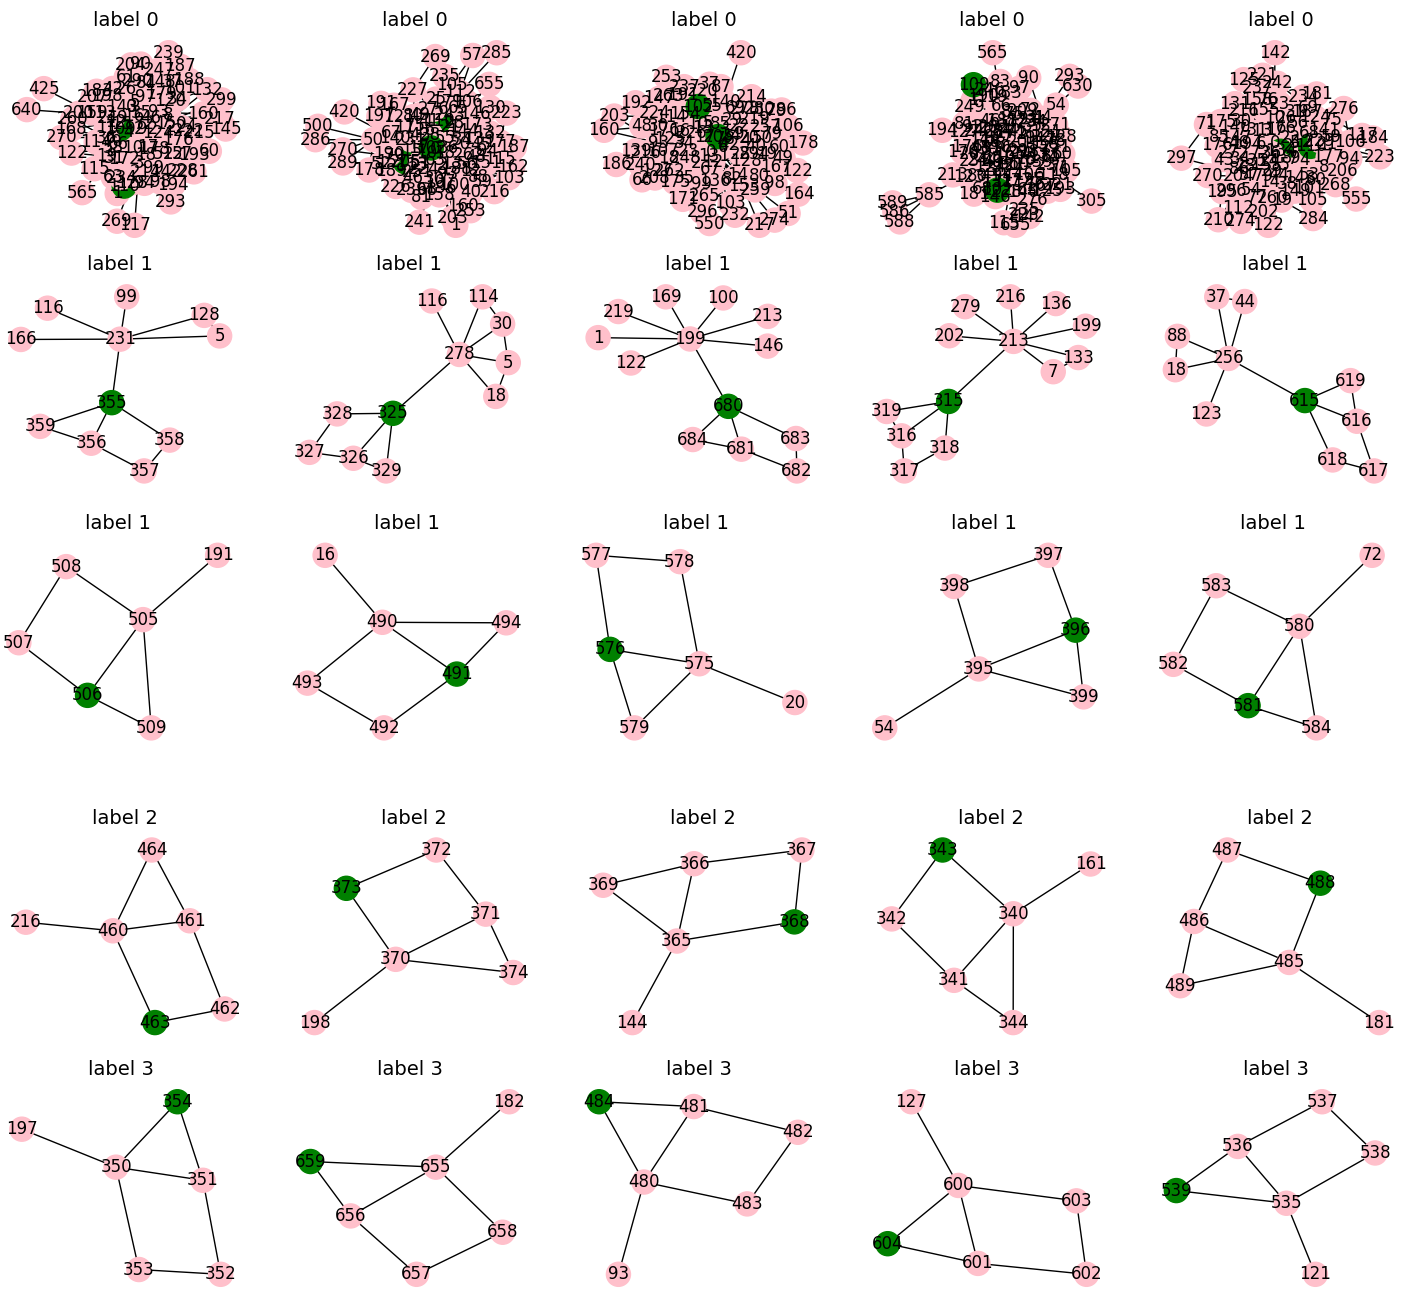
\includegraphics[width=0.45\textwidth]{figures/GCN-BA-Shapes}
    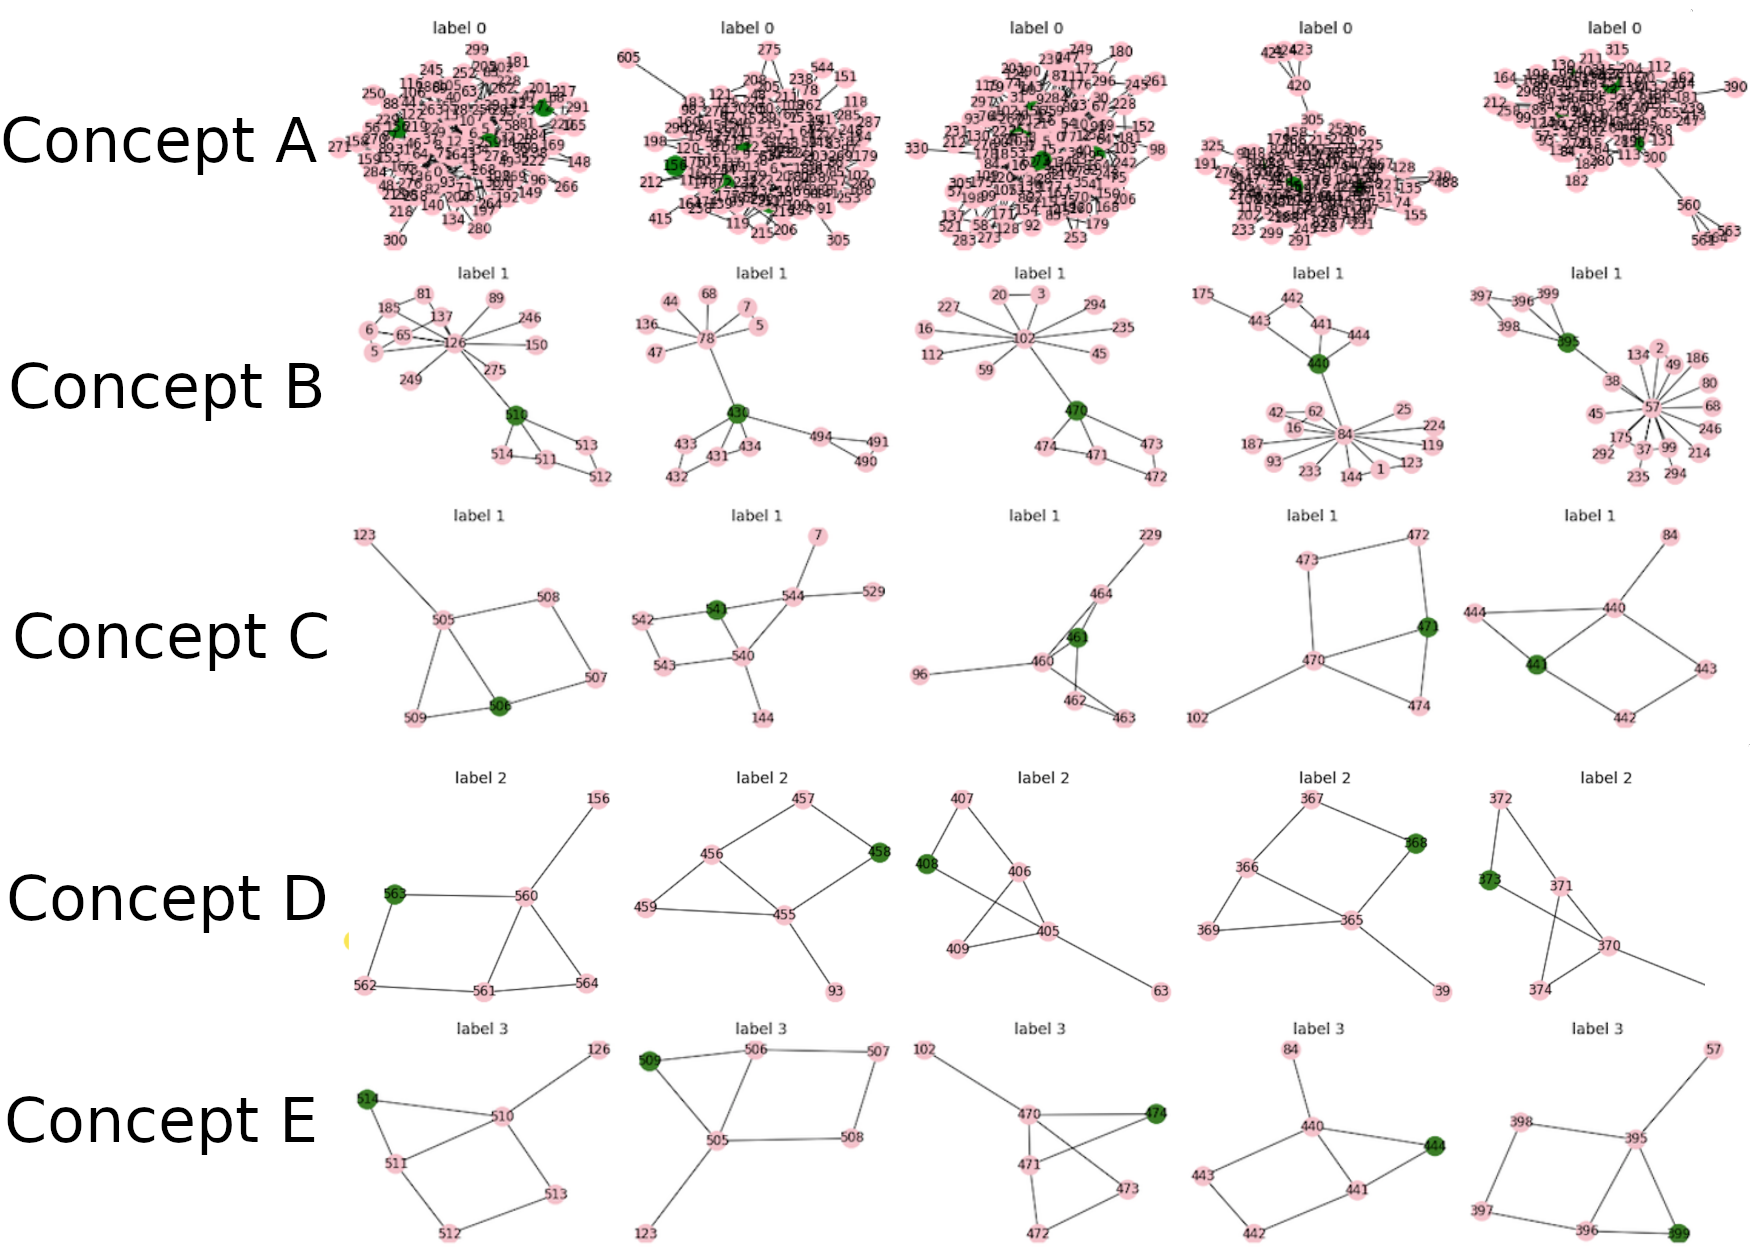
\includegraphics[width=0.45\textwidth]{figures/Magister-BA-Shapes}
    \caption{A subset of concepts discovered for BA-Shapes from the best perfomring GCN model compared to those published in figures 2, 3, and 5 in \textit{Magister et al.}\cite{magister2021gcexplainer}. Green nodes highlight the node of interest and pink nodes highlight the neighbourhood used for inference. Each row represents an individual concept.}
    \label{fig:GCN-BA-Shapes}
\end{figure}

%\fig{GCN-BA-Shapes}{A subset of concepts discovered for BA-Shapes from the best perfomring GCN model. Green nodes highlight the node of interest and pink nodes highlight the neighbourhood used for inference. Each row represents an individual concept.}
%
%\fig{Magister-BA-Shapes}{A subset of the BA Shapes concepts discovered in figures 2, 3 and 5 from \textit{Magister et al.}\cite{magister2021gcexplainer} to demonstrate the full range of labels. Each row represents an individual concept, the same colour system is used as fig. \ref{fig:GCN-BA-Shapes}.}

Figure \ref{fig:GCN-BA-Shapes} presents a comparison of BA Shapes concepts reproduced by the best performing GCN model and hose published in \textit{Magister et al.}
Concept 1 and A are included to demonstrate that the model does identify the base graph.
The remaining concepts demonstrate the 3 other labels associated with the house motif, as discussed in \Sref{sec:synth}.
All the published concepts have an equivalent concept in the reproduced concepts.
In both results the edge attaching the house motif to the base graph is important to the classification of the nodes.
The same distinction between concepts 2 and 3 as concepts B and C representing ``inside'' and the ``outside'' nodes respectively is also present in both.
%Notice that in both concept 2 and B the  ``inside'' node clearly attaches to the Barabasi-Albert base graph.
%This distinction is also present in concept 4 and D, with both the published and reproduced concepts focusing on the ``inside'' bottom node.

In both cases, and as expected given the concept purity scores, the concepts related to the motifs are almost completely pure with the exception of concept 1 and B.
Additionally, all the nodes in the house motif have a unique concept where applicable and this leads to the high completeness score.

Given the visual similarity in concepts between the published and reproduced results I consider the implementation of GCN to be accurate.
Examples of the other datasets are available in \Aref{app:concepts}.

\section{Comparison of Accuracy}
\label{sec:comp-acc}
\begin{table}
    \centering
    \begin{tabular}{c|c}
        \textbf{Dataset} & \textbf{Accuracy} \\
        \midrule
        BA Shapes       & 61.4\% $\pm$ 3.3 \\
        BA Grid         & 72.4\% $\pm$ 1.6 \\
        BA Community    & 20.6\% $\pm$ 1.5 \\
        Tree Cycles     & 50.5\% $\pm$ 4.2 \\
        Tree Grid       & 59.2\% $\pm$ 1.6 \\
    \end{tabular}
    \caption{Test accuracy in \% of SGC on each of the synthetic datasets using the hyperparameters in table \ref{tab:SGC-params}. As per \textit{Wu et al.}\cite{wu2019simplifying} outliers are removed as defined in \note{reference when complete}.}
    \label{tab:GCN-acc}
\end{table}



Table \ref{tab:SGC-acc} demonstrates the mean accuracies achieved by each of the SGC models using the hyperparameters in \ref{tab:SGC-params}.
As a comparison the accuracies achieved by GCN are presented beside them.
The performanace of SGC is very poor and so random guesses are included to demonstrate this.

\paragraph{Compared to GCN}
the accuracies achieved by SGC are significantly worse and go against \textit{Wu et al.}'s claim that SGC can match GCN perfomance.
In the majority of cases the accuracy achieved by SGC is roughly $50\%$ less than that achieved by GCN.
BA Grid, the highest performing dataset, achieves $72.4\%$ accuracy which is still $27.1\%$ less than GCN.
%does SGC achieve a good accuracy in comparison to GCN though even here the difference in accuracy is $27.1$\%.

These poor results suggest that the graph structure awareness of SGC is far worse than that of GCN as labels are based only on graph structure.
This is also an explanation for why SGC is able to surpass the accuracy of GCN in the Planetoid\cite{kipf2016semi} datasets as these datasets rely heavily on node representations.

\paragraph{Compared to random guesses}
SGC does not perform significantly better except in the cases of BA Shapes and BA Grid.
In the cases of the Tree datasets this can be attributed to the sparsity of the base graph where the motif structure and BST structure share similar connectivity.

In comparison the dense BA graph allows for a better distinction between the motifs and the base graph.
This distinction is attributed to the degree normalisation demonstrated in equation \ref{eq:GCN-as-GNN}.
This advantage is not present in BA Community the two communities and the possibility of a motif having multiple connections to different base graphs.

These results are not due to poor hyperparameter selection as demonstrated in \Aref{app:hyperparameters} and discussed in \Sref{sec:hyperparameters}.
Instead the explanation for the poor performance is due to the lack of proper graph structure awareness.

\paragraph{Comparison of parameters}
Given that SGC uses a single classifier layer compared to GCNs multiple layers there is a large discrepancy in the number of parameters\footnote{SGC has roughly 40 parameters compared to GCN with $>$1000 for BA Shapes.}.
However, increasing the parameters for SGC by either increasing the node feature size or adding a \emph{multi-layer perceptron}(MLP)\footnote{The use of an MLP classifier also introduces non-linearity though in this case the model does not improve. Non-linearity and parameters on there own are not sufficient.} with the same hidden layers as the GCN model results in no substantial change to accuracy.

No MLP model is added before the SGC pre-computation step as this defeats the point of linearisation.
This is the main drawback of SGC as it cannot manipulate the node representations except through filter application.
These claims are further explored in \Sref{sec:comp-concept}.

\section{Comparison of concepts}
\label{sec:comp-concept}

To achieve the \ref{crit1}$^{st}$ and \ref{crit3}$^{rd}$ success criterion concepts need to be extracted from SGC and compared to GCN concepts.
However, as stated before, concept extraction and analysis is only suggested for models that achieved $95$\% or higher on synthetic datasets by \textit{Ying et al.}\cite{ying2019gnnexplainer}.
As demonstrated in \Sref{sec:comp-acc} SGC does not reach this value only reaching $72.4$\% in the best case.

However, though the concepts will not be meaningful to explain how SGC reasons they will still provide insight into the claims in \Sref{sec:comp-acc}.
Furthermore, the concepts highlight the shortcomings of SGC when it comes to graph structure awareness.
For this reason the analysis of the concept scores is limited but the qualitative concept analysis provides insight into where SGC fails.

\paragraph{Success criterion}
Table \ref{tab:SGC-acc} demonstrates and implementation of SGC trained on the synthetic datasets with tables \ref{tab:SGC-completeness} and \ref{tab:SGC-purity} showing concept extraction.
Figures \ref{fig:SGC-BA-Shapes} and \ref{fig:BA-Community} visualise the extracted concepts from the relevant SGC model. These fulfill the \ref{crit1}$^{st}$ success criterion.

Table \ref{tab:SGC-completeness} and \ref{tab:SGC-purity} also include a comparison to the scores achieved by GCN.
\Sref{sec:comp-concept} includes a detailed analysis of the concepts extracted for SGC and comparison to those extracted for GCN.
These fullfil the \ref{crit3}$^{rd}$ success criterion.

\subsection{Quantitative analysis}
\label{sec:quant}
\paragraph{Completeness}
\begin{table}
    \centering
    \begin{tabular}{c|c|c}
        \textbf{Dataset} &
        \textbf{SGC} &
        \textbf{GCN} \\
        \midrule
        BA Shapes       & 0.882 & 0.964 \\
        BA Grid         & 0.843 & 1.000 \\
        BA Community    & 0.264 & 0.678 \\
        Tree Cycles     & 0.874 & 0.949 \\
        Tree Grid       & 0.890 & 0.965 \\
        \midrule
        Mutagenicity    & 0.537 & 0.967 \\
    \end{tabular}
    \caption{Concept completeness scores of SGC on each of the synthetic datasets using the hyperparameters in table \ref{tab:SGC-params} compared to the completeness scores of the equivalent GCN models.}
    \label{tab:SGC-completeness}
\end{table}



Table \ref{tab:SGC-completeness} demonstrates the completeness scores achieved by SGC compared to GCN and as expected, by the low accuracy achieved by SGC in \Sref{sec:comp-acc}, they are consistently lower than the equivalent GCN models.
However, given the accuracies of SGC appears closs to random, the resulting completeness scores aresurprisingly close to the GCN scores except in the case of BA Community.

The high completenes scores are due to the fact that completeness relates to importance of concepts and not the performance of the model.
The relatively high completeness scores for SGC signify that the concepts that SGC produces have some relevance to the class of a node.
However, as demonstrated by table \ref{tab:SGC-completeness}, this relevance is not as strong as that in GCN.

\paragraph{Purity}
\begin{table}
    \centering
    \begin{tabular}{c|ccc|c}
        \multirow{2}{*}{\textbf{Dataset}} &
        \multicolumn{3}{c}{\textbf{SGC}} & \\
        & \textbf{Max.} & \textbf{Min.} & \textbf{Mean} & \multirow{-2}{*}{\textbf{GCN}}\\
        \midrule
        BA Shapes       & 0.0 & 4.0 & 0.8 (5) & 0.000 (4) \\
        BA Grid         & 0.0 & 0.0 & 0.0 (2) & 0.000 (2) \\
        BA Community    & 0.0 & 6.0 & 4.0 (4) & 5.600 (3) \\
        Tree Cycles     & 0.0 & 6.0 & 1.0 (6) & 4.391 (9) \\
        Tree Grid       & 0.0 & 7.0 & 3.3 (10) & 1.417 (6) \\
    \end{tabular}
    \caption{Concept purity of SGC on each of the synthetic datasets using the hyperparameters in table \ref{tab:SGC-params} compared to the average purity achieved by the equivalent GCN model. The brackets represent the number of concepts considered for purity, as per \Sref{sec:evaluation} these are graphs with less than 13.}
    \label{tab:SGC-purity}
\end{table}



Table \ref{tab:SGC-purity} demonstrates the purity scores achieved by the best performing SGC model compared to GCN.
As discussed in \Sref{sec:GCN-reproduction} the values for purity are likely to be very erratic and not well suited for direct comparison.
Given this erratic behaviour the values for purity between the two approaches are somewhat correlated with SGC achieving fairly pure concepts.
As demonstrated SGC can identify pure concepts as is the case of BA Grid, which matches GCN in completely pure concepts.\footnote{For subgraphs the contain less than 13 nodes.}

However, the inclusion of the number of concepts considered when calculating purity demonstrates the limitation of this method of comparison.
Due to the base graphs a number of concepts contain more than 13 nodes and therefore are not considered.
Thus the pure concepts of BA Grid are not representative of all the concepts extracted.

Overall, this demonstrates that though SGC does not perform as well as GCN it produces concepts that are as coherent as GCN produces.

\subsection{Qualitative analysis}
\label{sec:concept-analysis}

\paragraph{BA Shapes}
\fig{SGC-BA-Shapes}{A subset of concepts extracted from the best performing SGC model. The subset includes both pure and impure concepts. The same colour scheme as fig. \ref{fig:GCN-BA-Shapes} is used.}

Figure \ref{fig:SGC-BA-Shapes} visualises a subset of the concepts extracted for SGC on BA Shapes.
Concepts 1 to 4 demonstrate the purer concepts extracted for SGC with concepts 5 to 7 representing the more common impure concepts.
Concept 5 demonstrates a shortcoming of calculating purity as this is considered a ``pure'' concept as the Barabasi-Albert graphs, having more than 13 nodes, are not considered. 
As with GCN, concept 1 demonstrates that SGC is able to identify the base graph.

Concepts 2, 3 and 4 demonstrate that SGC can identify pure concepts with important graph structure components.
These concepts can be directly compared to concepts 3, 2 and 4 in figure \ref{fig:GCN-BA-Shapes} respectively.
As with GCN the attaching arm is important to the classification of the nodes and there is some distinction between ``inside'' and ``outside'' nodes.
However, as can be seen in concept 2, this distinction is not as strong as GCN.

Concepts 5, 6 and 7 demonstrate the impure concepts that are extracted from SGC.
This is the major shortcoming of SGC it cannot consistently distinguish between the base graph and the motif.
%Given that the nodes of interest in house motif are all consistent across these concepts suggests that there is an element of structure being identified.
The problem is that SGC is unable to discern between structures that produce similar node representations.

These observations are hypothesised to be a result of limited learnable influence on node representations in SGC.
Though equation \ref{eq:theta} suggests that the GCN node manipulation should be preserved the reality is that only the final filter output is manipulated.
This observation leads to the extension presented in \Sref{sec:Jump-SGC} allowing SGC to access individual filter applications.

\paragraph{BA Community}
\begin{figure}
    \centering
    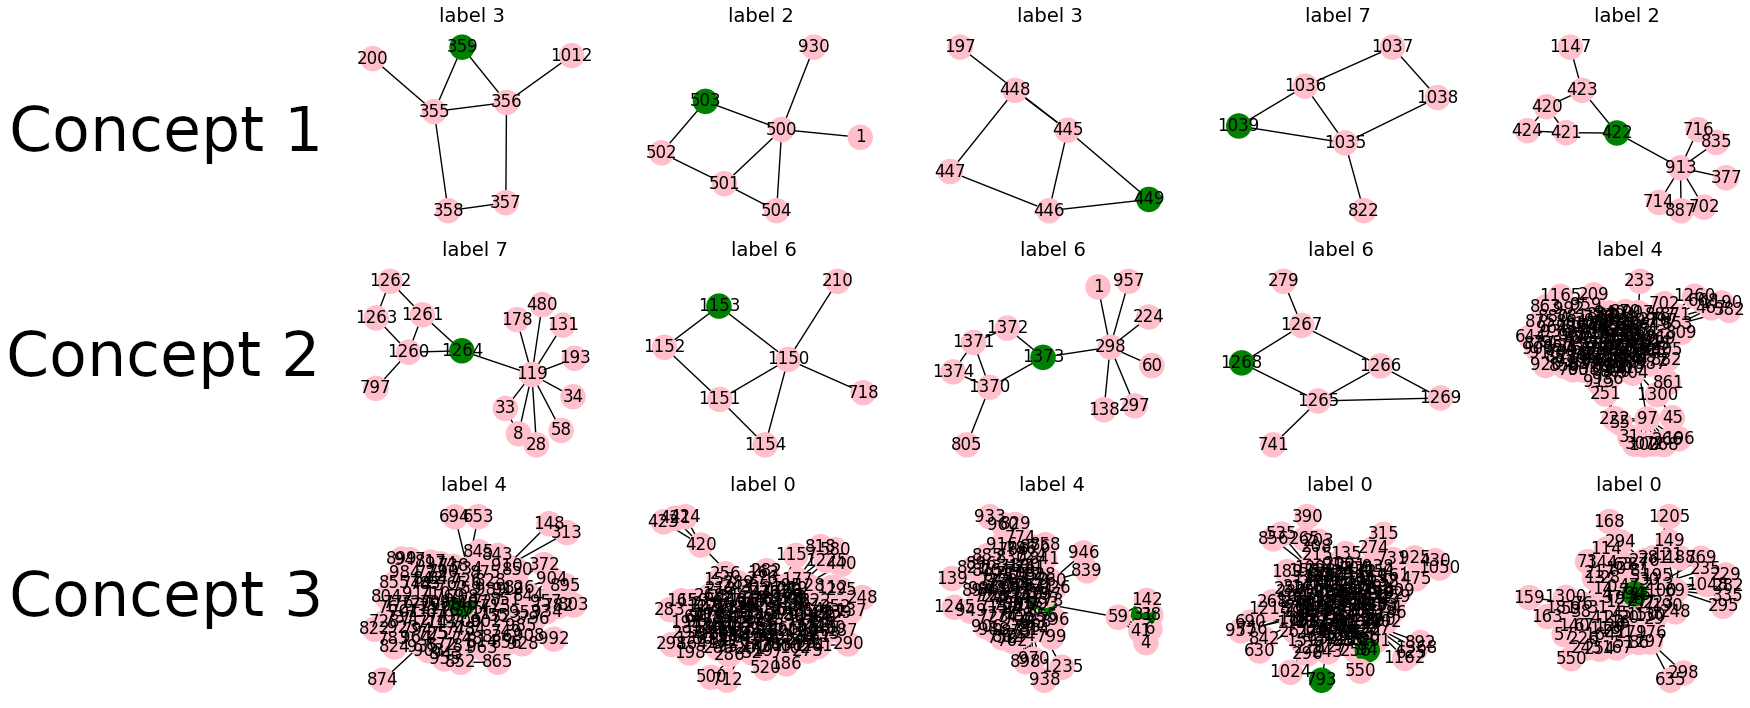
\includegraphics[width=0.75\textwidth]{figures/SGC-BA-Community}
    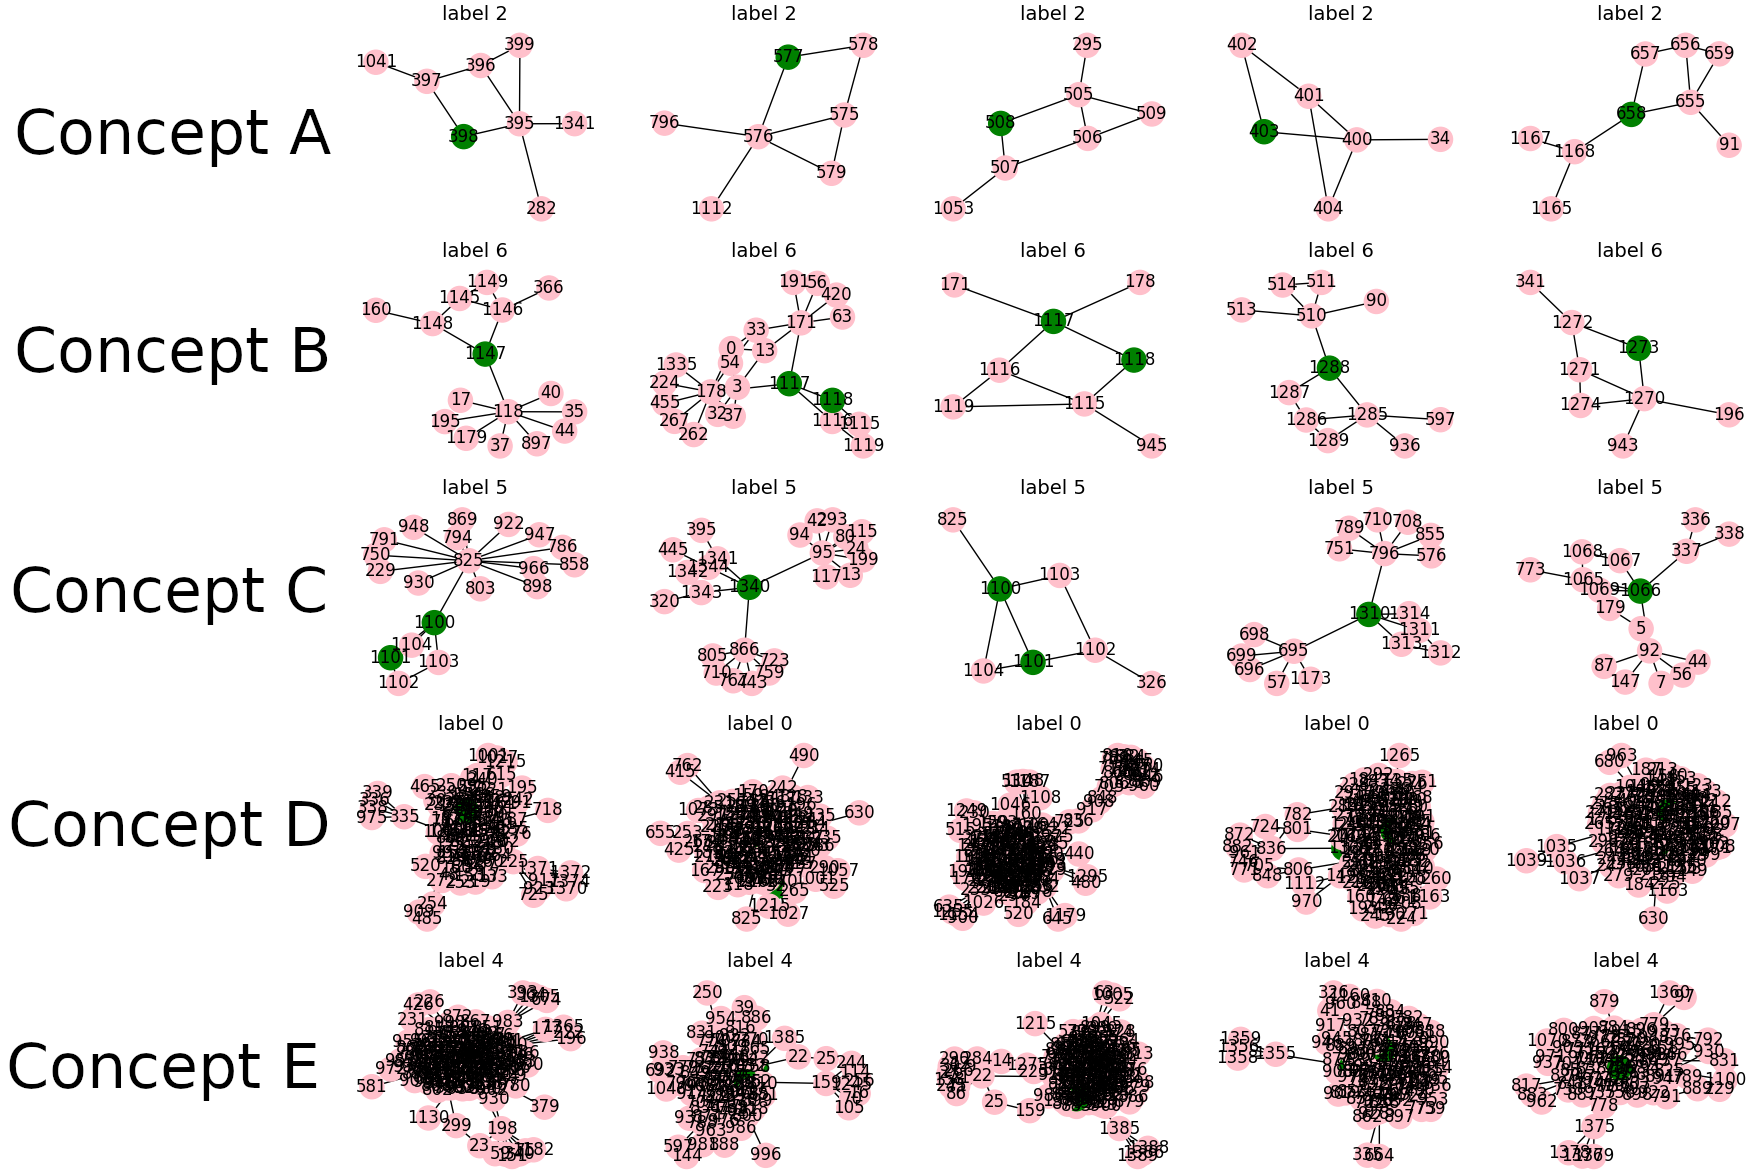
\includegraphics[width=0.75\textwidth]{figures/GCN-BA-Community}
    \caption{Comparison of SGC and GCN concepts for BA Community demonstrating the poor graph structural inference of SGC. The numbered concepts are a subset of SGC concepts and the lettered concepts are GCN concepts. The colour scheme is the same as fig. \ref{fig:GCN-BA-Shapes}.}
    \label{fig:BA-Community}
\end{figure}

Figure \ref{fig:BA-Community} highlights the inability of SGC to accurately discern graph structure where GCN demonstrate accurate graph structure awareness.
Concepts 1, 2 and 3 demonstrate the purer concepts for SGC trained on BA Community and Concepts A to E represent the equivalent concepts for GCN.

As discussed SGC may be able to identify graph structure, as shown in concepts 1 and 2, however concept 1 highlights the fact that SGC cannot determine which part of the graph structure a node is.
Comparatively concepts A, B and C show similar structures except consistent labels across the concept.

Furthermore, concept 2 groups nodes from the second community\footnote{labels 4, 5, 6 and 7.} together not nodes with the same graph structure.
In comparison, GCN is able to discern between members in the same community demonstrated by concepts B and C
Additionally, GCN can distinguish between different communities as concepts A and B represent the same node in the house motif but different communities.
%This erroneous behaviour is not standard as concept 3 highlights how the Barabasi-Albert subgraphs from separate communities are grouped together.
GCN treats the two communities different regardless of structural similarity which is clear in concepts D and E compared to concept 3.

Overall SGC is able to infer basic graph structure or group nodes into communities but is unable to achieve fine-grained awareness.
Though particularly apparent in BA Community these behaviours of SGC effect the performance on other datasets.

\subsection{Summary}
\note{I think this can be better worded, more detailed summary with a link back to introduction questions.}
The low accuracy of SGC means that the data present in tables \ref{tab:SGC-completeness} and \ref{tab:SGC-purity} does not carry much meaning.
However, table \ref{tab:SGC-completeness} does suggest that SGC does not produce useful concepts even though table \ref{tab:SGC-purity} suggests that these concepts are coherent.

When looking at the concepts produce it is clear that SGC is not a capable GNN for synthetic datasets.
Figures \ref{fig:SGC-BA-Shapes} and \ref{fig:BA-Community} highlight how the relatively good purity and completeness scores do not relate to useful concepts.
The linearisation of GCN clearly does not maintain the graph capabilities of GCN contrary to the results and claims of \textit{Wu et al.}.

Considering the large parameter disparity and adjusting SGC to compensate does not improve the performance.
This suggests that non-linearity and trainable parameters are important at specific points during inference not on their own.

\section{Extensions}
\label{sec:extension-eval}
\subsection{Evaluation}
All the extensions explored focus on improving the ability of SGC or expanding the functionality of the model.
Therefore to evaluate the success of these attempts the models are evaluated using the same techniques used in \ref{sec:evaluation}.
As these are extensions a smaller subset of the graph datasets are considered looking mainly at BA Shapes, as the best performing dataset, and BA Community, as the worst.

\subsection{SGC graph classification}
\label{SGC-graph}
\fig{SGC-Mutagenicity}{Concepts from SGC and GCN for Mutagenicity comparing the complexity of the inferred graph structure. The numbered concepts are a subset of SGC concepts and the lettered concepts are a subset of GCN. The colour scheme matches standard chemical colours.}

Tables \ref{tab:SGC-acc}, \ref{tab:SGC-completeness} and \ref{tab:SGC-purity} already include the results achieved by SGC on Mutagenicity.
The same quantitative analysis presented in \Sref{sec:quant} can be applied to the results achieved by SGC.
This suggests that the source of the graph data is not the issue, even though SGC performed well on Planetoid\cite{Fey/Lenssen/2019}.
As discussed in \Sref{sec:comp-acc} the cause for the discrepancy is due to Planetoid\cite{Fey/Lenssen/2019} being focused on node representation.
%Comparatively, Mutagenicity is both node representation and graph structure focused due to the nature of molecules.

Figure \ref{fig:SGC-Mutagenicity} further highlights the shortcomings of SGC compared to GCN.
Concepts 1, 2 and 3 focus on the inclusion of a single atom or small molecule structure wheres A, B and C demonstrate complex multi-atom structures.
Concepts 1 and 2 suggest identification structure though consistently focus on single atoms whereas concepts A and B show consistent multi-atom structures.
In the extreme concept 3 highlights the focus on grouping by atom, the major consistent feature the chlorine atom.
In comparison, concept C highlights how GCN is able to identify very large structures, two cyclic rings are consistently identified across all examples.

\subsection{SGC and GCN mixed model}
\label{sec:SGCN}
\fig{SGC-GCN-latent-space}{The 2D t-SNE reduced latent space of the first layer where SGC and GCN activations are most similar based on adjusted mutual information of their concepts. Concepts are calculated with the same number of clusters and receptive field.}
\fig{SGCN-SGC-latent-space}{The 2D t-SNE reduced latent space of the second layer where SGCN and SGC activations are most similar based on adjusted mutual information of their concepts. Concepts are calculated with the same number of clusters and receptive field.}
\fig{SGCN-GCN-latent-space}{The 2D t-SNE reduced latent space of the final (third) layer where SGCN and GCN activations are most similar based on adjusted mutual information of their concepts. Concepts are calculated with the same number of clusters and receptive field.}
\begin{table}[h]
    \centering
    \captionsetup{width=.9\textwidth}
    \begin{tabular}{c|c|cc}
        \textbf{Dataset} & \textbf{SGCN} & \textbf{SGC} & \textbf{GCN} \\
        \midrule
        BA Shapes       & 95.6\% $\pm$ 3.0 & 61.4\% $\pm$ 3.3 & 98.0\% $\pm$ 2.2 \\
    \end{tabular}
    \caption{Test accuracy in \% of SGCN on BA Shapes where the first layer is SGC precomputaion and the remaining two layers are GCN layers. The results achieved by SGC and GCN run for the same number of epochs are added as comparison.}
    \label{tab:SGCN-acc}
\end{table}


\begin{table}
    \centering
    \begin{tabular}{c|c|cc}
        \textbf{Model} & \textbf{Layer 1} & \textbf{Layer 2} & \textbf{Layer 3} \\
        \midrule
        GCN     & 0.736 & 0.743 & 0.926 \\
        SGC     & \underline{0.800} & 0.757 & 0.700 \\
        \midrule
        SGCN    & \underline{0.800} & \textbf{0.764} & \textbf{0.971} \\
    \end{tabular}
    \caption{Completeness scores for each of the layers of SGCN trained on BA Shapes where the first layer is SGC precomputaion and the remaining two layers are GCN layers. The results achieved by SGC and GCN run for the same number of epochs are added as comparison.}
    \label{tab:SGCN-completeness}
\end{table}



As the process of finding the optimal model, training and then evaluating said model requires many steps only BA Shapes is considered.
Figures \ref{fig:SGC-GCN-latent-space}, \ref{fig:SGCN-SGC-latent-space} and \ref{fig:SGCN-GCN-latent-space} show the t-SNE reduced latent space of the different models.
Tables \ref{tab:SGCN-acc} and \ref{tab:SGCN-completeness} demonstrate the results achieved by SGCN in both accuracy and concept completeness.

Figure \ref{fig:SGC-GCN-latent-space} demonstrates the first layer which has the highest AMI between GCN and SGC.
The similarity is not very high but is significantly higher than the similarity between SGC and GCN for the remaining layers.
This does present a potential issue in combining models where no significant mutual information is present.

Figure \ref{fig:SGCN-SGC-latent-space} demonstrates that the second layer of SGCN is very similar to that of SGC.
This is due to the previous layer being an SGC layer and so the GCN layer applied to a different feature space.
The spread green labelled nodes (representing the house motif ``floor'') is also present in the GCN layers in \ref{fig:SGC-GCN-latent-space} and \ref{fig:SGCN-GCN-latent-space} demonstrating a mixture of representation.
Figure \ref{fig:SGCN-GCN-latent-space} shows that the final layer of SGCN has a latent space that is very similar to that of GCN.
Given the increase in performance by SGCN demonstrated in table \ref{tab:SGCN-acc} this likely to be a more optimal space.

Though SGCN does not surpass the performance of GCN as shown in table \ref{tab:SGCN-acc} it is able to surpass it in completeness score highlighted in table \ref{tab:SGCN-completeness}.
This happens across all layers (noting that the first layer is identical to the SGC layer) and highlights a major benefit of the model.
GCN takes all 3 layers to reach a high completeness score whereas SGC starts high but then decreases as more layers are added.
By combining the layers the completeness score to remains high throughout.

An analysis of the concepts extracted for SGCN are presented in \Sref{app:concepts}.

\subsection{Jumping knowledge SGC}
\label{sec:Jump-SGC}

\begin{table}
    \centering
    \begin{tabular}{c|c|cc}
        \textbf{Dataset} & \textbf{JSGC} & \textbf{SGC} & \textbf{GCN} \\
        \midrule
        BA Shapes       & 78.2\% $\pm$ 3.2 & 61.4\% $\pm$ 3.3 & 98.0\% $\pm$ 2.2 \\
        BA Community    & $\pm$ & 20.6\% $\pm$ 1.5 & 86.3\% $\pm$ 3.3 \\
    \end{tabular}
    \caption{Test accuracy in \% of JSGC on a subset of synthetic datasets using the hyperparameters in table \note{reference when complete}. Each experiment is run until convergence. Results from SGC and GCN are provided as a comparison.}
    \label{tab:SJGC-acc}
\end{table}


\begin{table}[h]
    \centering
    \captionsetup{width=.9\textwidth}
    \begin{tabular}{c|c|cc}
        \textbf{Dataset} &
        \textbf{JSGC} &
        \textbf{SGC} &
        \textbf{GCN} \\
        \midrule
        BA Shapes       & 0.943 & 0.882 & 0.964 \\
        BA Community    & \textbf{0.704} & 0.264 & 0.678 \\
    \end{tabular}
    \caption{Concept completeness scores of JSGC on a subset of the synthetic datasets using the hyperparameters in table \ref{tab:JSGC-params} compared to the completeness scores of the equivalent SGC and GCN models. Each model is run until convergence and the best performing model selected for concept extraction.}
    \label{tab:JSGC-completeness}
\end{table}


\begin{table}[h]
    \centering
    \captionsetup{width=.9\textwidth}
    \begin{tabular}{c|ccc|cc}
        \multirow{2}{*}{\textbf{Dataset}} &
        \multicolumn{3}{c|}{\textbf{JSGC}} & \\
        & \textbf{Max.} & \textbf{Min.} & \textbf{Mean} & 
        \multirow{-2}{*}{\textbf{SGC}} &
        \multirow{-2}{*}{\textbf{GCN}}\\
        \midrule
        BA Shapes       & 0.0 & 0.0 & 0.0 (2) & 0.8 (5) & 0.000 (4) \\
        BA Community    & 4.0 & 16.0 & 9.4 (7) & 4.0 (4) & 5.600 (3) \\
    \end{tabular}
    \caption{Concept purity of JSGC on a subset of the synthetic datasets using the hyperparameters in table \ref{tab:JSGC-params} compared to the average purity achieved by the equivalent SGC and GCN model. The brackets represent the number of concepts considered for purity, as per \Sref{sec:evaluation} these are graphs with less than 13.}
    \label{tab:JSGC-purity}
\end{table}



Tables \ref{tab:JSGC-acc}, \ref{tab:JSGC-completeness} and \ref{tab:JSGC-purity} show the results achieved by JSGC on the datasets analysed in \Sref{sec:comp-concept}.
Overall these demonstrate that JSGC does outperform SGC significantly and is more comparable to GCN.
The accuracy achieved by JSGC is still lower than the the 95\% suggested by \textit{Ying et al.}\cite{ying2019gnnexplainer} but significantly better.
This improvement is seen in table \ref{tab:JSGC-completeness} as the completeness scores are closer to 1 with BA Community producing better performing concepts than GCN.\footnote{This is partially a result of the concept parameters used. The high score signifies that good concepts are being utilised by the model but in this case the model still does not appear to be quite capable enough.}
The purity presented in table \ref{tab:JSGC-purity} is higher though more concepts were considered and BA Community is a very complex graph.

\fig{JSGC-BA-Community}{A subset of concepts from JSGC for BA Community demonstrating the improved graph structure awareness. The concepts are chosen to represent the GCN concepts presented in \ref{fig:BA-Community}. The colour scheme is the same as fig \ref{fig:GCN-BA-Shapes}.}

Figure \ref{fig:JSGC-BA-Community} highlights the improvements that JSGC has made compared to SGC.
Comparing these concepts to those achieved by GCN presented in figure \ref{fig:BA-Community} shows a clear improvement.
Concepts 1 to 5 in fig. \ref{fig:JSGC-BA-Community} can be directly mapped to A to E in fig. \ref{fig:JSGC-BA-Community}.\footnote{A similar direct mapping was also achieved for BA Shapes.}
JSGC is now able to distinguish between the two communities highlighted by concepts 1 \& 2 and 3 \& 4.
Furthermore, within a community JSGC correctly distinguishes between the different nodes as concept 2, 3 and 4 show.
Most importantly all concepts, except for concept 1, show consistent labelling throughout, particularly in concept 3 where all nodes are ``outside''\footnote{See \Sref{sec:concept-analysis}.} nodes.

Clearly JSGC has comparable graph structure awareness as GCN and does not require the non-linearity of GCN to achieve this.
The lower accuracy of JSGC still suggests that there are elements of GCN that are important to its success and generally GRL.
However, further studies into the importance of non-linearity in GRL is required.

\chapter{Conclusion}

\section{Summary}
This dissertation set out to analyse how linearising GNN architectures match the performance of their non-linear counterparts.
%It aimed to understand how graph structure can be better utilised by analysing these two approaches.
%This was achieved by comparing graph concepts from GCN and its linear counterpart, SGC.
As \Sref{sec:comp-acc} demonstrated the linear GNN, SGC, does not match the performance of its non-linear counterpart.
\Sref{sec:comp-concept} highlights the poor graph structure awareness of SGC suggesting that non-linearity is key to inferring structure.
Extending SGC to graph classification also shows the same lack of graph structure awareness.

To combat these limitations SGC and GCN are combined to utilise the benefits of both approaches.
However, though this is successful the use of SGC is very limited with the GCN layers providing the majority of the inference.

JSGC provides a novel extension to SGC with promising results highlighted in \Sref{sec:Jump-SGC} demonstrating graph structure awareness with an improvement of up to $50\%$ in accuracy compared to SGC.
JSGC provides SGC with intermediate node representations through the techniques present in JKNs~\cite{xu2018representation} allowing for influence and thus structural inference.
This demonstrates the performance of GNNs lies in manipulating and utilising the graph topology and from the non-linearity as is the case for standard NNs.
Importantly JSGC is negligibly non-linear demonstrating that graph structure awareness is possible within a linear architecture.

\section{Lessons learned}
My project aimed to understand the effect that linearising GNN architectures had on performance through graph concepts.
This effect depends as much on the dataset, the method of GNN explainability, and architecture as it does on the method of linearization.
Regardless, the project explored an area of this space and provided important insights.

Importantly, as shown by the proposed JSGC architecture, it is possible to achieve high graph structure awareness, achieving completeness scores of $0.943$ nearly reaching maximum completeness, whilst remaining negligibly non-linear.
This presents a new avenue of GNN architecture design outside of the standard deep learning approach and has utility in efficient graph structure inference.
But, as demonstrated by the poor performance of SGC, care must be taken in producing linear architectures to retain graph structure awareness.

The project did however demonstrate that non-linearity does provides higher accuracy when compared to linear architectures (GCN beats quasi-linear methods by at least $10\%$ and fully linear methods by $\approx 40\%$).
The results presented do not suggest that linear NNs are ideal but rather that graph structure awareness may be achieved through linear GNNs.
This distinction is highlighted by the poor performance of SGC and JSGC's inability to match the accuracy of GCN whilst achieving comparable graph structure awareness.
These drawbacks may potentially be solved by utilising more complex classifiers such as MLPs.

%The key skill learnt during the project was time management including careful planning allowing for unforeseen setbacks.
%Quick adaptation throughout was key as the majority of the project was research focused requiring exploration based on results.
%Maintaining good software practices and results loggin allowed for easier pivoting throughout the project.
%
%Saving all of the results that I had achieved throughout the project in a presentable format both helped quickly identify interesting results but also speed up the writing process.
%This is also true for keeping all the configuration files including those during experimentation as I was able to review past experiments when more knowledge was gained.
%Keeping notes on all the papers I read was also very useful however in future I would keep a better log of thoughts throughout the project.
%
%NN models are very sensitive to the hyperparameters used which can have a large impact on the apparent performance.
%The process of finding hyperparameters is very tedious as a large search space needs to be explored to verify that the chosen hyperparameters are optimal within that space.
%automating this process was very useful however I completed this process late in my project to verify the results that I had achieved are the best possible configuration.
%Though carrying out hyperparameter sweeps on all of my models did not effect the final analysis in future I will complete this step much earlier.

\section{Future work}
\paragraph{JSGC}
Graph structure awareness has been shown within a quasi-linear model suggesting that the current approach to GNN architecture may be overly complex.
The capabilities and limitations of JSGC have not been explored fully in this dissertation but the results in \Sref{sec:Jump-SGC} are worthy of further consideration.
%Though the accuracy of JSGC is not as high as GCN it is important to note that JSGC uses only 350 parameters compared to GCN's $>$1000 on BA Shapes.
Though the performance of JSGC is low (GCN beats JSGC by at least $16\%$) it may be best utilised in conjunction with more sophisticated classifiers separating graph structure inference from node label inference.

\paragraph{AMI mixed models}
To combine SGC and GCN the extracted concepts are compared using AMI to determine where the two approaches are similar.
As demonstrated in \Sref{sec:SGCN-eval} in figure \ref{fig:SGCN-latent-spaces} the resulting model retains the influence of both models.
%\textit{Shchur et al.}~\cite{shchur2018pitfalls} and \textit{Purchase et al.}~\cite{purchase2022revisiting} demonstrate the best performing GNN is highly dependent on training setup and dataset.
By combining the best-performing GNN models in different environments using the AMI approach it may be possible to overcome the individual GNN limitations.

\paragraph{Other GNN architectures}
Multiple GNN architectures have been proposed which achieve high accuracy on many benchmark datasets.
However, there have been limited attempts to understand how the architectures achieve high performance outside of theoretical proofs.
Applying explainability tools, such as \textit{GCExplainer}~\cite{magister2021gcexplainer}, will provide further insight and present possible areas of improvement.


\appendix
\chapter{Proposal}
\section{Description}

\subsection{Introduction}

Within the area of geometric deep learning there have been recent ablation studies looking into the effectiveness of Graph Neural Networks (GNNs). The majority of these studies question the effectiveness of the deep neural network approach of multiple layers separated by non-linear function passes when working with geometric datasets (graphs). \cite{wu2019simplifying} introduce a new approach, Simplified Graph Convolution (SGC), which remove these non-linear functions from the network. This reduces the problem to a pre-computation on the graph adjacency matrix and a simple linear regression using a single weight matrix. The pre-computation on the graph adjacency matrix encodes information about message passing between nodes in the graph.  \cite{chanpuriya2022simplified} introduce further variations on SGC that use the same underlying concept of a pre-computation but deal with the parameters differently allowing for more complex associations. In both cases the results show that removing the non-linearity does not hinder the performance of the network and can in fact improve performance.

Similarly, the has been a lot of interest into explainable artificial intelligence (XAI) to move away from the black box nature of AI models. There exists multiple methods within this field of machine learning and I will specifically focus on the idea of Concepts. Concepts focuses on relating specific outputs of a model to subspaces within its input space, this gives an indication of what the model is using within the input space to infer the given output. The collections of these subspaces are what are known as concepts. This approaches allows a human actor to get a better understanding of the model's inference as they can compare their own intuition of the input to the concepts the model uses to produce the given result.
\cite{magister2021gcexplainer} introduce GCExplainer which adapts prior techniques to extract high-level concepts from GNNs. The paper focuses on extracting concepts from a Graph Convolutional Network (GCN, \cite{kipf2016semi}) model.

Both SGC and GCExplainer are research papers but both including detailed sections on experiment setup and available github repositories. In the case of GCExplainer the author of the paper is one of my supervisors and can therefore clear up any setup details and help with common pitfalls in the training process.

\subsection{Extensions}

Further extensions on the core goal will look at the concepts extracted from variations on SGC with potential new approaches outside of existing literature being implemented. Approaches outside of literature include mixing SGC "layers" within GCN layers, allowing for non-linearity to be added later in the forward pass. Equally using multiple SGC steps and using Jump Knowledge \cite{xu2018representation} to help combat the common problem of over-smoothing in GNNs. Further extensions may be found based on results during the project.

These extensions can also look into how accurate the new models are outside of the concept metrics and provide further comparison between accuracy and concept purity \& completeness.

\subsection{Substance and Structure}

With the rise in popularity of simplified GNNs due to their simple nature and effective representational learning it is important to evaluate how they fit into explainability frameworks. This project therefore looks to extract concepts from SGC trained on the same datasets using in \cite{magister2021gcexplainer} to compare against GCN. This work will provide useful insight into how these simplified networks operate as well as providing further comparison between previous GNN techniques (GCN) and new simplified GNN techniques (SGC). Comparison between the two GNN techniques will focus on concept purity and completeness as described in \cite{magister2021gcexplainer}.

This is broken down into reproducing both papers using the setup and structure described in each to compare the results that I achieve with those published in each paper. The code used for both of these can then be combined to extract concepts from the SGC model. This will allow comparison between a simplified GNN (SGC) and a standard GNN (GCN). Further extensions can then be carried out based on these results to further investigate different GNN approaches in regard to concept extraction. 

\section{Starting Point}

I have worked with Pytorch and the extension for geometric deep learning, Pytorch Geometric, over the summer culminating in a research paper. During this summer project I worked with building and testing graph datasets, building new GNN models, and testing/comparing GNN models from previous models to the new models. During the project I also briefly learnt about and used convolutional neural networks and transformers. I do not have experience with XAI or the area of Concepts.

No code has been written for this project beyond the code that will be used within the Pytorch and Pytorch Geometric libraries.

\section{Success Criteria}

The project will be deemed a success if I 

\begin{itemize}[noitemsep]
    \item Implement SGC and extract the concepts used for each of the datasets
    \item Implement GCN and extract the concepts to use as a baseline
    \item Compare the concepts between SGC and GCN using the metrics of concept completeness and concept purity
\end{itemize}

\section{Work Plan}

\subsection{Interval 1: 13/10 - 26/10}

\textit{Preparatory Work:} Download datasets (both SGC and GCExplainer), preliminary tests on datasets to check all correct, setup up environment (required libraries are up-to-date etc.), test training on local machine and servers to determine extra resources. Read and annotate the three papers being implemented.

Start work on implementing Simplified Graph Convolution (SGC).

\subsection{Interval 2: 27/10 - 9/11}

Complete implementation of SGC and train on SGC paper datasets, compare against papers results to confirm implementation is correct. Train SGC on GCExplainer datasets.

\textbf{Milestone:} Trained SGC model.

\textit{Category Theory 1 Deadline: 4/11 (25\%)}

\subsection{Interval 3: 10/11 - 23/11}

Implement Graph Convolution Network (GCN, from GCExplainer) and train on GCExplainer datasets.

\subsection{Interval 4: 24/11 - 7/12}

Implement GCExplainer concept extraction on GCN and compare concept metrics to confirm implementation is correct.

\textbf{Milestone:} Working GCExplainer.

\textit{Category Theory 2 Deadline: 2/12 (75\%)}

\subsection{Interval 5: 8/12 - 21/12}

Carry out concept extraction on the trained SGC model(s) and produce concept metrics for SGC model(s).

\textbf{Milestone:} SGC concept metrics (\textbf{Core Project Complete})

\subsection{Interval 6: 22/12 - 4/1}

\textit{Buffer.} Christmas and New Year

\subsection{Interval 7: 5/1 - 18/1}
\label{interval:extension}

\textit{Extension:} Research (read papers and annotate) one of the following techniques

\begin{itemize}[noitemsep]
    \item Mixing SGC and GCN layers
    \item Adding knowledge jumps
    \item Other simplified graph convolutions
\end{itemize}

\subsection{Interval 8: 19/1 - 1/2}

\textit{Extension:} Implement and train the chosen technique from \Cref{interval:extension} on the GCExplainer Datasets.

\subsection{Interval 9: 2/2 - 15/2}

\textit{Extension:} Carry out GCExplinaer concept extraction on the trained model from \Cref{interval:extension}.

\textbf{Deadline:} Progress Report 3/2

\subsection{Interval 10: 16/2 - 1/3}

\textit{Write Dissertation:} Introduction and Implementation chapters, and share with supervisors.

\textit{Deep Neural Networks 1 Deadline: 17/02 (30\%)}

\subsection{Interval 11: 2/3 - 15/3}

\textit{Buffer.} If not required and extension runs smoothly carry out a second technique from \Cref{interval:extension}.

\subsection{Interval 12: 16/3 - 29/3}

\textit{Write Dissertation:} Evaluation of different approaches and their concept metrics, and share with supervisors.

\textbf{Milestone:} First draft

\subsection{Interval 13: 30/3 - 12/4}

\textit{Write Dissertation:} Respond to feedback on first draft and share with supervisors.

\textbf{Milestone:} Second draft

\textit{Deep Neural Networks 2 Deadline: 17/03 (70\%)}

\subsection{Interval 14: 13/4 - 27/4}

\textit{Write Dissertation:} Respond to feedback on second draft and share with supervisors.

\textbf{Milestone:} Final draft

\textbf{Deadline:} Dissertation submission 12/5

\section{Supervisors}

\begin{itemize}[noitemsep]
    \item Lucie Charlotte Magister
    \item Pietro Babiero
    \item Pietro Lio
\end{itemize}

I will have joint weekly meetings at 5pm on Wednesday will all supervisors (barring temporary unavailability) to report on the progress of the project and help with any problems that have occurred in the current interval. 

\section{Resource Declaration}

My own machine (AMD Ryzen 7 5700U with Radeon Graphics (16) @ 1.8GHz, 16GB RAM, and AMD ATI Lucienne) for the primary implementation of the project and remote work on any provided servers used. The majority of the project should be completed on this machine. I will also use git version control storing a remote repository on a private github repository in the eventuality of my own machine malfunctioning. Regular remote pushes at the end of the day or major project milestones will be carried out. I accept full responsibility for this machine and I have made contingency plans to protect myself against hardware and/or software failure.

High performance cluster (HPC) as intensive training may be required. The required hours will remain within the SL3 bracket so no funding for SL2 will be required. 

Local CL server access (idun, heimdall, etc) for less costly iterations and testing of GPU models before utilising HPC if my own machine is not sufficient. I am able to acquire kerberos tickets to use these services.

Storage space available on my own machine will be sufficienet for the datasets used. Though space on local CL and HPC servers would be required if I am using these for model training.

I will require other software packages, PyTorch and PyTorch Geometric, to help with the framework of building, testing and training my models.


%\bibliography{references}

%\end{document}


\bibliography{references}

\end{document}
